\documentclass[conference]{IEEEtran}
\IEEEoverridecommandlockouts
% The preceding line is only needed to identify funding in the first footnote. If that is unneeded, please comment it out.
\usepackage{cite}
\usepackage{amsmath,amssymb,amsfonts}
\usepackage{algorithmic}
\usepackage{graphicx}
\usepackage{array}
\usepackage{textcomp}
\usepackage[table]{xcolor}
\usepackage{multirow}
\usepackage{multicol}
\usepackage{float}
\usepackage[utf8]{inputenc}
\usepackage[vietnamese]{babel}
\usepackage{amsmath}
\usepackage[T5]{fontenc}
\usepackage{titlesec}
\usepackage{tabularx}
\usepackage{adjustbox}

\titlespacing*{\subsubsection}{0pt}{\baselineskip}{\baselineskip}

\def\BibTeX{{\rm B\kern-.05em{\sc i\kern-.025em b}\kern-.08em
    T\kern-.1667em\lower.7ex\hbox{E}\kern-.125emX}}
\title{Sử dụng kỹ thuật phân tích Chuỗi thời gian vào bài toán dự đoán giá Cổ phiếu}
\author{\IEEEauthorblockN{1\textsuperscript{st} Nông Tiến Dũng}
\IEEEauthorblockA{\textit{{IS304.O21.VN}} \\
\textit{Đại học Công nghệ Thông tin}\\
20521213@gm.uit.edu.vn}
\and
\IEEEauthorblockN{2\textsuperscript{nd} Đỗ Văn Sáng}
\IEEEauthorblockA{\textit{IS304.O21.VN} \\
\textit{Đại học Công nghệ Thông tin}\\
20521832@gm.uit.edu.vn}
\and
\IEEEauthorblockN{3\textsuperscript{rd} Tạ Quang Hưng}
\IEEEauthorblockA{\textit{IS304.O21.VN} \\
\textit{Đại học Công nghệ Thông tin}\\
21520036@gm.uit.edu.vn}
\and
\IEEEauthorblockN{4\textsuperscript{th} La Hoài Nam}
\IEEEauthorblockA{\textit{IS304.O21.VN} \\
\textit{Đại học Công nghệ Thông tin}\\
20521629@gm.uit.edu.vn}
\and
\IEEEauthorblockN{5\textsuperscript{th} Nguyễn Quang Huy}
\IEEEauthorblockA{\textit{IS304.O21.VN} \\
\textit{Đại học Công nghệ Thông tin}\\
20521403@gm.uit.edu.vn}
}
\begin{document}
\maketitle

\begin{abstract}
Bài báo sử dụng kỹ thuật phân tích chuỗi thời gian trong bài toán dự đoán giá cổ phiếu. 
Dự đoán giá cổ phiếu là một tác vụ khó khăn do tính phức tạp và biến động của thị trường tài chính. 
Trong bài báo, chúng tôi sử dụng các mô hình:
SEMOS, Random Forest, Fuzzy for predict times series, LightGBMModel, ResCNN, Linear regression, 
Autoregressive Integrated Moving Average (ARIMA), Recurrent Neural Networks (RNN), Gated recurrent units (GRU)
và Long Short-Term Memory (LSTM) để dự đoán giá cổ phiếu trên ba bộ dữ liệu AbbVie, AstraZeneca và Pfizer. 
Sau đó thực hiện so sánh hiệu suất của các mô hình dựa trên ba độ đo: RMSE, MSE và MAPE.
\end{abstract}

\begin{IEEEkeywords}
Cổ phiếu, SEMOS, Random Forest, Fuzzy for predict times series, LightGBMModel, ResCNN, Linear regression, ARIMA, RNN, GRU, LTSM
\end{IEEEkeywords}

\section{GIỚI THIỆU}
Cổ phiếu được coi là hình thức đầu tư trọng điểm trong ngành tài chính, đại diện cho quyền sở hữu một phần trong tổ chức phát hành. Theo Investopedia, công ty Đông Ấn Hà Lan phát hành cổ phiếu đầu tiên vào năm 1602 tại Sở Giao dịch Chứng khoán Amsterdam, đồng thời cũng là công ty đầu tiên phát hành cổ phiếu và trái phiếu. Điều này đã được coi là một sự tiến bộ quan trọng trong lĩnh vực tài chính và đã mở ra thời kỳ phát triển của thị trường cổ phiếu.

Định giá cổ phiếu là quy trình xác định giá trị thị trường thực sự của cổ phiếu tại một thời điểm nhất định, nhằm hiểu rõ tiềm năng của cổ phiếu để đưa ra quyết định đầu tư phù hợp. Đối với doanh nghiệp, việc định giá cổ phiếu được coi là một trong những bước tiên quyết khi công ty cổ phần dự định phát hành cổ phiếu, huy động vốn và tăng cường ảnh hưởng của mình trên thị trường. Từ góc độ của nhà đầu tư, việc định giá cổ phiếu giúp họ xác định cổ phiếu nào đáng để đầu tư và có tiềm năng mang lại lợi nhuận tối đa.

Một phương pháp tiếp cận sơ bộ trong việc định giá cổ phiếu là đánh giá giá trị cổ phiếu. Nếu giá cổ phiếu hiện tại thấp hơn giá trị đã định giá, nhà đầu tư có thể xem xét mua cổ phiếu. Ngược lại, nếu giá cổ phiếu vượt quá giá trị đã định giá và nhà đầu tư hiện đang sở hữu cổ phiếu, họ có thể bán cổ phiếu để thu về lợi nhuận.

Thực tế cho thấy có nhiều thuật toán và kỹ thuật hỗ trợ việc dự báo giá cổ phiếu của ba doanh nghiệp bao gồm: Catalent, Intel Corporation, Nutrien. Trong nghiên cứu này, chúng tôi sẽ áp dụng 10 mô hình: SEMOS, Meta-Learning, Fuzzy for predict time series, LightGBMModel, ResCNN, Linear regression, ARIMA, RNN, GRU, LSTM để tiến hành đánh giá hiệu suất các mô hình, sau đó sử dụng hai mô hình tốt nhất thực hiện dự đoán giá đóng cửa của cổ phiếu trong 30 ngày, 60 ngày và 90 ngày tiếp theo. 

\section{CÁC NGHIÊN CỨU LIÊN QUAN}
Zou Xiaowu và đồng nghiệp cung cấp các phương pháp dựa trên CNN cho Phân loại Chuỗi Thời gian (TSC) [1] và các hàm kích hoạt được sử dụng. Một MC-CNN được đề xuất cho phân loại chuỗi thời gian đa biến. Phương pháp này trích xuất đặc trưng bằng cách sử dụng nhiều CNN khác nhau và kết hợp chúng. một CNN đa quy mô.

Guolin Ke và đồng nghiệp đề xuất hai kỹ thuật mới là Gradient-based One-Side Sampling (GOSS) và Exclusive Feature Bundling (EFB). GOSS tập trung vào việc loại bỏ một phần lớn các mẫu dữ liệu có độ dốc thấp, trong khi EFB gom nhóm các đặc trưng phân biệt để giảm số lượng đặc trưng. Cả hai kỹ thuật này nhằm tối ưu hóa hiệu suất huấn luyện của GBDT và giảm thiểu thời gian tính toán [2].

European Centre for Medium-Range Weather Forecasts (ECMWF) sử dụng mô hình EMOS để cải thiện dự báo thời tiết từ mô hình dự báo số học [3]. Việc áp dụng EMOS đã giúp ECMWF cải thiện độ chính xác của dự báo thời tiết, đặc biệt là ở các kỳ vọng ngắn và trung hạn.

Trong một nghiên cứu được công bố vào năm 2007, Chin-Teng Lin và đồng nghiệp đã sử dụng mô hình Fuzzy Time Series để dự đoán huyết áp trong tương lai dựa trên các giá trị huyết áp trong quá khứ [5]. Mô hình này sử dụng các tập luật Fuzzy để mô hình hóa mối quan hệ giữa các biến số đầu vào và đầu ra. Kết quả của nghiên cứu cho thấy rằng mô hình Fuzzy có khả năng dự đoán chuỗi thời gian của huyết áp một cách chính xác và hiệu quả, giúp trong việc theo dõi sức khỏe của bệnh nhân và đưa ra các biện pháp phòng ngừa kịp thời.

Nhóm tác giả Vaishnavi Gururaj, Shriya V R và Dr. Ashwini K [6] đã nghiên cứu về thị trường chứng khoán bằng mô hình Linear Regression. Dataset mà nhóm tác giả sử dụng là một năm dữ liệu cổ phiếu của Công ty Coca-Cola, từ 01/2017-2018. Các kết quả về độ đo bao gồm: 3.22 (RMSE), 2.53 (MAE), 10.37 (MSE) và 0.73 (R-Squared).

Nghiên cứu "Performance analysis of machine learning models for intrusion detection system using Gini Impurity-based Weighted Random Forest (GIWRF) feature selection technique"[7], tác giả Raisa Abedin Disha và S. Waheed đã thử nghiệm và đánh giá hiệu suất của các mô hình học máy như GRU và GBT trong việc phân loại trong hệ thống phát hiện xâm nhập. Các mô hình này đã được huấn luyện và kiểm tra trên hai tập dữ liệu UNSW-NB 15 và Network TON\_IoT. Để tăng cường hiệu suất của các mô hình, tác giả đã sử dụng kỹ thuật lựa chọn đặc trưng gọi là Gini Impurity-based Weighted Random Forest (GIWRF). Kỹ thuật này giúp tác giả chọn ra một tập hợp tối ưu các đặc trưng từ dữ liệu. Kết quả thực nghiệm cho thấy mô hình Cây quyết định (DT) hoạt động tốt hơn so với các mô hình khác trong thí nghiệm này khi sử dụng kỹ thuật lựa chọn đặc trưng GIWRF.

Box và Jenkins đã giới thiệu mô hình ARIMA vào năm 1970. Đây còn được gọi là phương pháp Box-Jenkins, bao gồm một tập hợp các hoạt động để xác định, ước lượng và chẩn đoán các mô hình ARIMA với dữ liệu chuỗi thời gian [8]. Các mô hình ARIMA đã chứng minh khả năng tạo ra dự đoán ngắn hạn hiệu quả. ARIMA liên tục vượt trội so với các mô hình phức tạp khác trong dự đoán ngắn hạn [9].

Ba tác giả Murtaza Roondiwala, Harshal Patel và Shraddha Varma đã áp dụng mô hình LSTM (Long Short-Term memory) trong việc dự đoán giá trị của cổ phiếu của NIFTY 50 [10]. Họ đã sử dụng 500 epochs để train và kết quả đạt được là vô cùng tốt. Mô hình cho ra được các kết quả RMSE trên tập test rơi vào khoảng 0.00859. Sai số vô cùng thấp cho thấy giá trị dự đoán cực kì tốt.

Tác giả Yongqiong Zhu [11] đã sử dụng mô hình RNN để dự đoán giá cố phiếu của Apple với dữ liệu huấn luyện là giá cổ phiểu của Apple (AAPL) trong 10 năm (từ 9/8/2009 đến 12/8/2020 với tập train chiếm 65\% và tập test chiếm 35\% còn lại. Tác giả đã xây dựng mô hình mạng RNN hai lớp với lớp thứ nhất có 50 nút đơn vị và lớp thứ hai chứa 100 nút đơn vị. Tác giả sử dụng 50 epochs, tối ưu hóa bằng Adam và dùng hàm mất mát là MSE đã cho ra được một kết quả rất tốt. Mô hình cho kết quả độ chính xác của dự đoán lên đến hơn 95\% và giá trị mất mát là 0.1\%.

\section{TÀI NGHUYÊN}
\subsection{DỮ LIỆU}
Bài báo sử dụng bộ dữ liệu được lấy từ dữ liệu chứng khoán của 3 công ty ABBV 
(Dữ liệu của công ty AbbVie được lấy về từ trang web finance.yahoo.com có 1259 dòng dữ liệu), AZN 
(Dữ liệu của công ty AstraZeneca được lấy về từ trang web finance.yahoo.com có 1259 dòng dữ liệu) 
và PFE (Dữ liệu của công ty Pfizer được lấy về từ trang web finance.yahoo.com có 1259 dòng dữ liệu). 
Với dữ liệu được thu thập từ ngày 1/3/2019 đến ngày 01/06/2024 và được tải về vào ngày 24/06/2024. 
Ở cả 3 bộ dữ liệu đều có các cột thuộc tính liên quan đến cổ phiếu.

\begin{table}[H]
  \centering
  \caption{Mô tả thuộc tính trong ba bộ dữ liệu}
\begin{tabular}{|>{\columncolor{red!20}}c|c|}
    \hline
     \rowcolor{red!20} Thuộc tính & Mô tả\\ \hline
     Date & Ngày diễn ra giao dịch \\ \hline
     Open & Giá cổ phiếu đầu tiên được giao dịch\\ \hline
     High & Giá cao nhất của cổ phiếu được giao dịch\\ \hline
     Low & Giá thấp nhất của cổ phiếu được giao dịch\\ \hline
     Close & Giá đóng cửa của cổ phiếu\\ \hline
     Adj Close & Giá đóng của điều chỉnh\\ \hline
     Volume & Khối lượng giao dịch\\ \hline
\end{tabular}
\end{table}
\subsection{CÁC ĐỘ ĐO CHẤT LƯỢNG}
Chúng tôi đánh giá hiệu suất của các mô hình dự báo bằng ba chỉ số chính: Sai số trung bình bình phương (RMSE), Sai số trung bình tuyệt đối (MAE), và Sai số trung bình tuyệt đối phần trăm (MAPE), đảm bảo kiểm thử chính xác và toàn diện.

RMSE (Sai số trung bình bình phương): RMSE đại diện cho căn bậc hai của sai số trung bình bình phương giữa các giá trị dự báo và quan sát được. Nó thường được sử dụng trong phân tích hồi quy và dự báo, đặc biệt là khi độ chính xác là quan trọng. Giá trị RMSE thấp hơn chứng tỏ mức độ chính xác cao hơn trong các dự đoán của mô hình.

MAE (Sai số trung bình tuyệt đối): MAE đo lường độ lớn trung bình của sai số trong một tập hợp các dự đoán, bất kể chúng có phải là sự đánh giá cao hơn hay thấp hơn so với giá trị thực tế. Nó đánh giá hiệu quả của một mô hình hồi quy bằng cách tính trung bình khác biệt tuyệt đối giữa các giá trị dự đoán và các giá trị thực tế.

MAPE (Sai số trung bình tuyệt đối phần trăm): MAPE đánh giá độ chính xác dưới dạng phần trăm và được xác định là trung bình khác biệt phần trăm tuyệt đối giữa các giá trị dự đoán và các giá trị thực tế cho mỗi khoảng thời gian.

Công thức của RMSE:
\[RMSE=\sqrt{\sum_{i=1}^{n} \frac{(\hat{y_i}-y_i )^2}{n} }\]

Công thức của MAE:
\[MAE=\frac{1}{n}  \sum_{i=1}^{n} |y_i-\hat{y_i} |\]

Công thức của MAPE:
\[MAPE=\frac{1}{n}  \sum_{i=1}^{n} |\frac{y_i-\hat{y_i}}{y_i}|\]
Trong đó:\\
	\indent\textbullet\ \(n\) số lượng quan sát trong dữ liệu.\\
	\indent\textbullet\ \(y_i\)  giá trị thực tế của điểm dữ liệu thứ i.\\
	\indent\textbullet\ \(\hat{y_i}\) giá trị dự đoán của điểm dữ liệu thứ i.

\section{PHƯƠNG PHÁP}
\subsection{LINEAR REGRESSION}
Trong lĩnh vực thống kê, Linear Regression là một phương pháp dùng để xác định mối quan hệ giữa một biến phụ thuộc có giá trị số và một hoặc nhiều biến độc lập.

Khi chỉ có một biến độc lập, chúng ta gọi là hồi quy tuyến tính đơn giản (Simple Linear Regression). Trong trường hợp có nhiều biến độc lập, ta gọi là hồi quy tuyến tính đa biến (Multiple Linear Legression)

Simple Linear Regression được mô tả qua công thức:
\[
 y = \beta_0 + \beta_1 x + \varepsilon
\]
Trong đó:\\
	\indent\textbullet\ \(y\) : biến phụ thuộc (dependent variable) cần dự đoán.\\
	\indent\textbullet\ \(x\) : biến độc lập (independent variable) được sử dụng để dự đoán giá trị của y.\\
        \indent\textbullet\ $\beta_0$ : hệ số góc (intercept) của đường hồi quy, đại diện cho giá trị dự đoán của y khi x = 0.\\
        \indent\textbullet\ $\beta_1$ : hệ số hồi quy (regression coefficient), đại diện cho mức độ thay đổi của y dựa trên mỗi đơn vị thay đổi của x.\\
        \indent\textbullet\ $\varepsilon$: lỗi ngẫu nhiên (random error), biểu thị sự không thể tránh khỏi của mô hình trong việc mô phỏng dữ liệu thực tế.
\subsection{GRU}
GRU là một loại mạng thần kinh hồi quy dựa trên LSTM được tối ưu hóa đặc biệt, Đơn vị bên trong GRU tương tự như đơn vị bên trong LSTM, ngoại trừ việc GRU kết hợp cổng đến và cổng quên trong LSTM thành một cổng cập nhật duy nhất.
Mặc dù nó được lấy cảm hứng từ đơn vị LSTM, nhưng nó được coi là đơn giản hơn để tính toán và thực hiện. Nó duy trì khả năng miễn dịch LSTM đối với vấn đề độ dốc biến mất. Cấu trúc bên trong của nó đơn giản hơn và do đó, nó cũng dễ đào tạo hơn, vì cần ít tính toán hơn để nâng cấp các trạng thái bên trong. Cổng cập nhật kiểm soát mức độ thông tin trạng thái từ thời điểm trước đó được giữ lại ở trạng thái hiện tại, trong khi cổng đặt lại xác định xem trạng thái hiện tại có nên được kết hợp với thông tin trước đó hay không.
\begin{align*}
Z_t &= \sigma(x_t W^z + h_{t-1} U^z + b_z) \\
r_t &= \sigma(x_t W^r + h_{t-1} U^r + b_r) \\
\tilde{h}_t &= \tan(r_t \times h_{t-1} U + x_t W + b) \\
h_t &= (1 - z_t) \times \tilde{h}_t + z_t \times h_{t-1}
\end{align*}

\(W^z\), \(W^r\), W biểu thị các ma trận trọng số cho vectơ đầu vào được kết nối tương ứng.\(U^z\), \(U^r\), U đại diện cho ma trận trọng số của bước thời gian trước đó và $b_r$, $b_z$, b là sai lệch. Các $\sigma$ biểu thị chức năng sigmoid logistic, $r_t$ biểu thị cổng đặt lại, $z_t$ biểu thị cổng cập nhật và $\tilde{h}_t$ biểu thị lớp ẩn ứng cử viên.
\begin{figure}[H]
    \centering
    \begin{minipage}{0.5\textwidth}
    \centering
    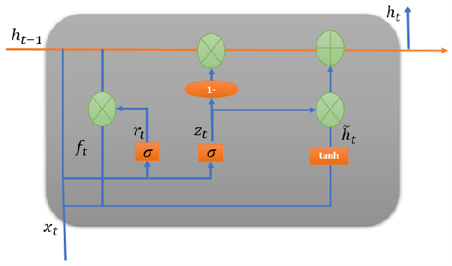
\includegraphics[width=1\textwidth]{Image/GRU.png}
    \label{fig:1}
    \end{minipage}
\end{figure}
\subsection{ARIMA}
Trong một mô hình ARIMA, giá trị tương lai của một biến được giả định là một hàm tuyến tính của một số quan sát quá khứ cộng với các lỗi ngẫu nhiên. Hàm tuyến tính này dựa trên ba thành phần tham số: tự hồi quy (AR), tích hợp sai phân (I) và trung bình trượt (MA). Mô hình ARIMA có thể được ký hiệu là ARIMA(p, d, q), trong đó p là số lượng thành phần tự hồi quy, d là số lượng sự khác biệt không mùa và q là số lượng lỗi dự báo trễ trong phương trình dự đoán. Giá trị tương lai của một biến trong ARIMA được biểu thị như sau:\\

\( y(t) = \varnothing_0 + \varnothing_1 y_{t-1} + \varnothing_2 y_{t-2} + \ldots + \varnothing_p y_{t-p} + \varepsilon_t - \theta_1 \varepsilon_{t-1} - \theta_2 \varepsilon_{t-2} - \ldots - \theta_q \varepsilon_{t-q} \) \\

Trong đó:\\
	\indent\textbullet\ \(y_t\) : giá trị thực tế.\\
	\indent\textbullet\ $\varepsilon_t$: sai số ngẫu nhiên tại thời điểm t.\\
        \indent\textbullet\ $\varnothing_i$ và $\varnothing_j$ : các hệ số.\\
\subsection{RNN}
Mạng neural hồi quy (RNN) là một mạng neural nhân tạo được thiết kế để xử lý dữ liệu chuỗi hoặc dữ liệu có mối quan hệ thời gian. Mạng RNN có khả năng lưu trữ thông tin từ quá khứ và sử dụng nó để dự đoán các giá trị trong tương lai.

Cấu trúc chính của mạng RNN là có một chuỗi các "đơn vị hồi quy" (recurrent units) được kết nối với nhau theo chiều thời gian.\\
\begin{figure}[H]
    \centering
    \begin{minipage}{0.5\textwidth}
    \centering
    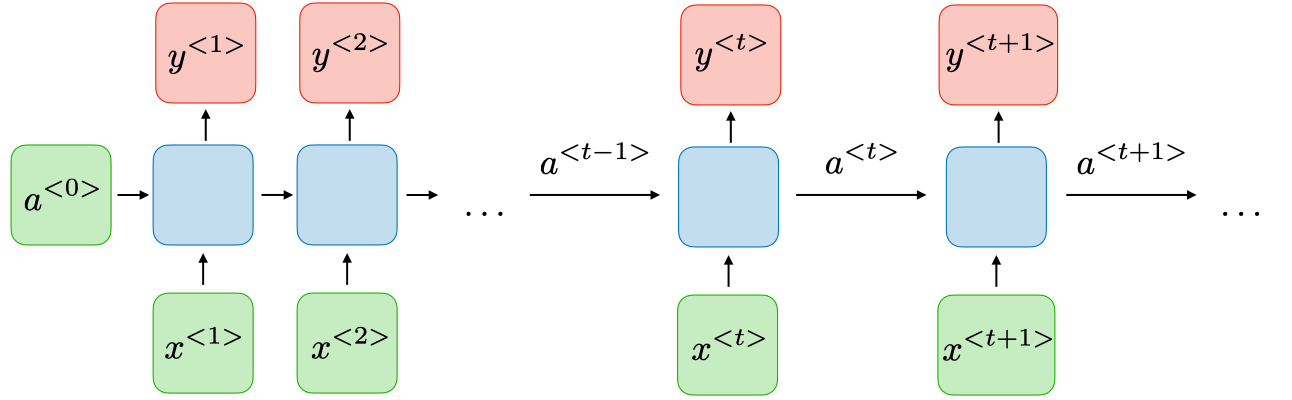
\includegraphics[width=1\textwidth]{Image/RNN1.png}
    \label{fig:1}
    \end{minipage}
\end{figure}

Đối với mỗi timestep t, giá trị kích hoạt \(a^{<t>}\) và đầu ra \(y^{<t>}\) được thể hiện như sau:
\[a^{<t>} = g_1(W_{aa}a^{<t-1>} + W_{ax}x^{<t>} + b_a)\]
\[y^{<t>} = g_2(W_{ya}a^{<t>} + b_y)\]

\begin{figure}[H]
    \centering
    \begin{minipage}{0.5\textwidth}
    \centering
    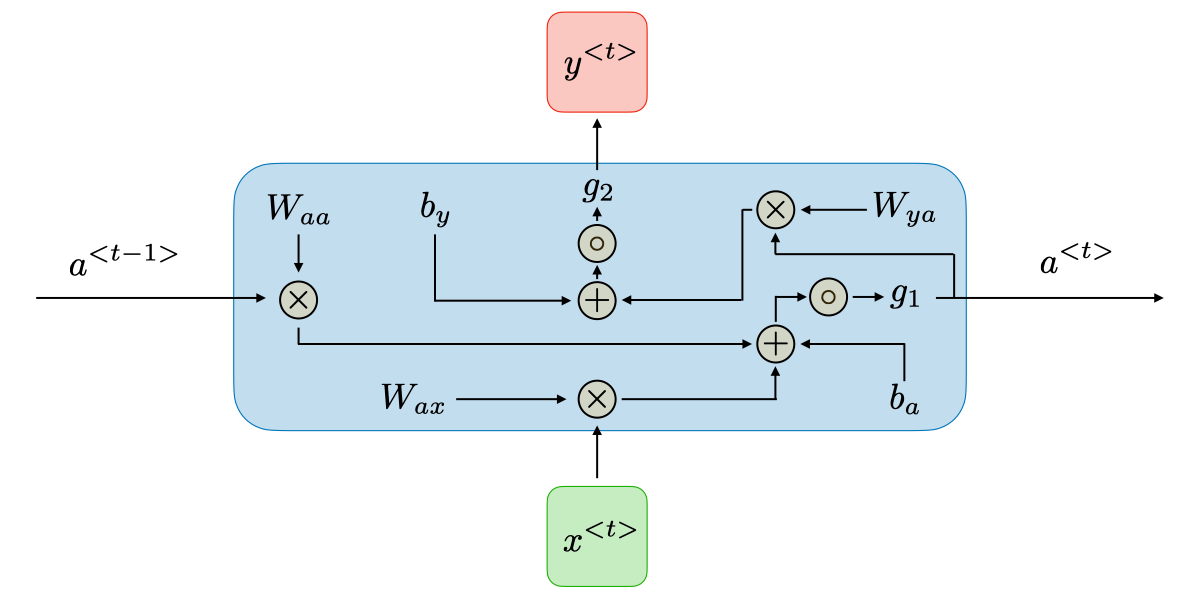
\includegraphics[width=1\textwidth]{Image/RNN2.png}
    \label{fig:1}
    \end{minipage}
\end{figure}
Trong đó:\\
	\indent\textbullet\ \(a^{<t>}\) : giá trị kích hoạt tại thời điểm t. \\
	\indent\textbullet\ \(y^{<t>}\) : giá trị đầu ra (dự đoán) tại thời điểm t. \\
 	\indent\textbullet\ \(x^{<t>}\) : giá trị đầu vào tại thời điểm t. \\
 	\indent\textbullet\ \(g_1\), \(g_2\) : là các hàm kích hoạt (activation function). \\
 	\indent\textbullet\ \(g_1\), \(g_2\) : là các hàm kích hoạt (activation function). \\
   	\indent\textbullet\ \(W_{aa}\), \(W_{ax}\), \(W_{ya}\) : lần lượt là các trọng số của giá trị kich hoạt, đầu vào và đầu ra của mô hình. \\
   	\indent\textbullet\ \(b_a\), \(b_y\): lần lượt là các giá trị bias của mô hình. \\
\subsection{LSTM}
Theo Alex Graves và đồng nghiệp (2005) [18] LSTM là viết tắt của "Long Short-Term Memory", một loại mạng nơ-ron học sâu hay còn được biến đến là một loại đặc biệt của mạng Recurrent Neural Network (RNN).

Một LSTM layer bao gồm một tập hợp các khối nhớ được kết nối theo chu kỳ. Mỗi khối chứa một hoặc nhiều ô nhớ được kết nối theo chu kỳ thông qua ba cổng nhân tích - cổng đầu vào, cổng đầu ra và cổng quên. Chúng cung cấp các phép ghi, đọc và đặt lại liên tục cho ô nhớ.

Sự ra đời của LSTM đã giúp hạn chế phần nào vấn đề phụ thuộc xa mà RNN mắc phải nhờ khả năng học các phụ th uộc dài hạn.

Cấu trúc của LSTM:
\begin{figure}[H]
    \centering
    \begin{minipage}{0.5\textwidth}
    \centering
    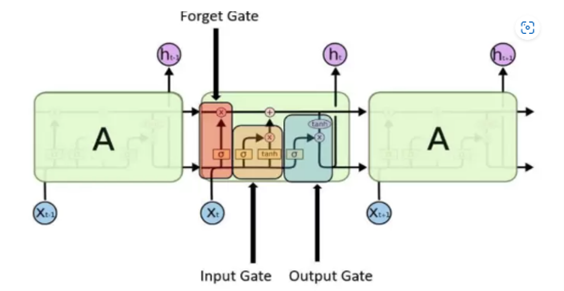
\includegraphics[width=1\textwidth]{Image/LSTM.png}
    \caption{Kiến trúc LSTM}
    \label{fig:1}
    \end{minipage}
\end{figure}
Công thức tính toán các cổng trong LSTM:\\
Forget gate: $f_t = \sigma(W_f \cdot x_t + U_f \cdot h_{t-1})$\\
Input gate: $i_t = \sigma(W_i \cdot x_t + U_i \cdot h_{t-1})$\\
Cell gate: $\tilde{c}_t = \tanh(W_c \cdot x_t + U_c \cdot h_{t-1})$\\
Output gate: $o_t = \sigma(W_o \cdot x_t + U_o \cdot h_{t-1})$\\
Cell state: $c_t = f_t \cdot \tilde{c}_t + i_t \cdot c_{t-1}$
\subsection{SEMOS}
SEMOS (Smooth EMOS) là một mô hình được đề xuất bởi Lang và các cộng sự (2020) để dự báo phân phối của một biến ngẫu nhiên \(Y\) có dạng phân phối chuẩn với trung bình và phương sai thay đổi theo thời gian. Mô hình SEMOS sử dụng các spline hồi quy chu kỳ để mô phỏng sự biến đổi theo mùa trong các tham số phân phối của biến.
Cụ thể, mô hình SEMOS có các phương trình như sau:

 Trung bình của phân phối tại thời điểm \(t\), \(\mu_S(t)\):
    \[\mu_S(t) := a_0 + f_0(t) + (a_1 + f_1(t)) \cdot x(t)\]
    \[= a_0 + f_0(t) + f_1(t) \cdot x(t) + a_1 \cdot x(t),\]
    trong đó \(f_0(t)\) và \(f_1(t)\) là các hàm spline hồi quy chu kỳ.

Log-phương sai của phân phối tại thời điểm \(t\):
    \[\log(\sigma_S(t)) := b_0 + g_0(t) + (b_1 + g_1(t)) \cdot s(t)\]
    \[= b_0 + g_0(t) + g_1(t) \cdot s(t) + b_1 \cdot s(t),\]
    trong đó \(g_0(t)\) và \(g_1(t)\) là các hàm spline hồi quy chu kỳ.

Các hàm spline hồi quy chu kỳ \(f_i(t)\) và \(g_i(t)\) được định nghĩa dựa trên chuỗi Fourier bị cắt ngắn, với các hệ số được tối ưu hóa thông qua việc tối thiểu hóa CRPS (Continuous Ranked Probability Score).

Mô hình SEMOS được thiết kế để nắm bắt hiệu ứng theo mùa và xu hướng trong dữ liệu dự báo, đồng thời có khả năng dự báo phân phối của biến ngẫu nhiên một cách chính xác hơn.

\subsection{RANDOM FOREST (RF)}
Random Forest là một phương pháp học máy kết hợp rộng rãi được sử dụng vì tính linh hoạt, đơn giản và thường mang lại kết quả chất lượng. Về bản chất thì Random Forest là tập hợp của nhiều cây quyết định, thay vì phụ thuộc vào một cây, nó lấy dự đoán từ mỗi cây và dựa trên đa số phiếu dự đoán, dự đoán kết quả cuối cùng.

Một cây quyết định được tạo thành từ ba loại nút:\\
	\indent Nút quyết định : Loại nút này có hai nhánh trở lên. \\
	\indent Các nút lá : Các nút thấp nhất đại diện cho quyết định. \\
 	\indent Nút gốc : Đây cũng là nút quyết định nhưng ở cấp cao nhất. \\
Random Forest là một thuật toán học có giám sát có thể giải quyết cả các vấn đề phân loại và hồi quy. Random Forest sử dụng nhiều cây quyết định tổng hợp để giúp tạo ra các dự đoán ổn định và chính xác hơn. Nó hoạt động theo bốn bước:
\\
	\indent\textbullet\ 1.	Chọn mẫu ngẫu nhiên từ tập dữ liệu cho trước. \\
	\indent\textbullet\ 2.	Thiết lập một cây quyết định cho mỗi mẫu và nhận kết quả dự đoán từ mỗi cây quyết định. \\
 	\indent\textbullet\ 3.	Sau đó, bỏ phiếu cho mỗi kết quả dự đoán. \\
 	\indent\textbullet\ 4.	Chọn kết quả được dự đoán nhiều nhất là kết quả dự đoán cuối cùng. \\
Dưới đây là mô hình của Random Forest:
\begin{figure}[H]
    \centering
    \begin{minipage}{0.5\textwidth}
    \centering
    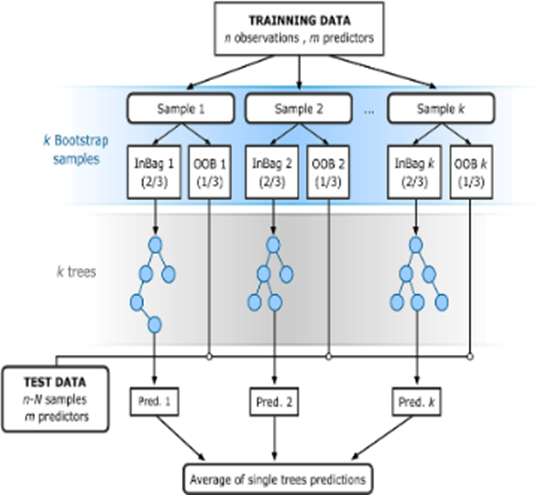
\includegraphics[width=1\textwidth]{Image/RF2.png}
    \label{fig:1}
    \end{minipage}
\end{figure}

\subsection{LIGHTGBMMODEL}
LightGBM là một thuật toán được phát triển bởi tổ chức Microsoft Research Asia dựa trên phương pháp cây quyết định tăng cường (Gradient Boosting Decision Tree (GBDT)) [26]. Một trong những ưu điểm của mô hình này là hiệu quả tính toán cao, đặc biệt đối với các bài toán dự đoán với số lượng lớn dữ liệu đầu vào. LightGBM sử dụng "histogram-based algorithms" thay thế cho "pre-sort-based algorithms" thường được dùng trong các boosting tool khác để tìm kiếm split point trong quá trình xây dựng tree. Cải tiến này giúp LightGBM tăng tốc độ training, đồng thời làm giảm bộ nhớ cần sử dụng. 
\begin{figure}[H]
    \centering
    \begin{minipage}{0.5\textwidth}
    \centering
    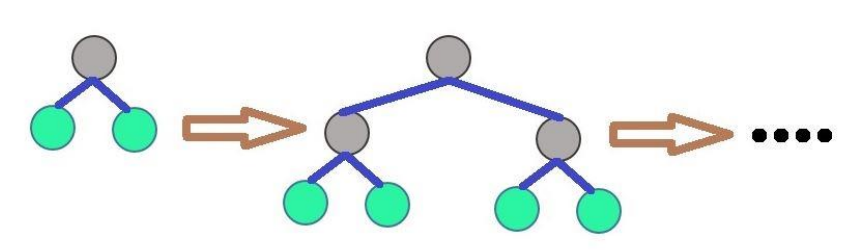
\includegraphics[width=1\textwidth]{Image/Level-wise Tree Growth.png}
    \caption{Chiến lược tăng trưởng theo độ sâu của cây (Level-wise Tree Growth)}
    \label{fig:1}
    \end{minipage}
\end{figure}
\begin{figure}[H]
    \centering
    \begin{minipage}{0.5\textwidth}
    \centering
    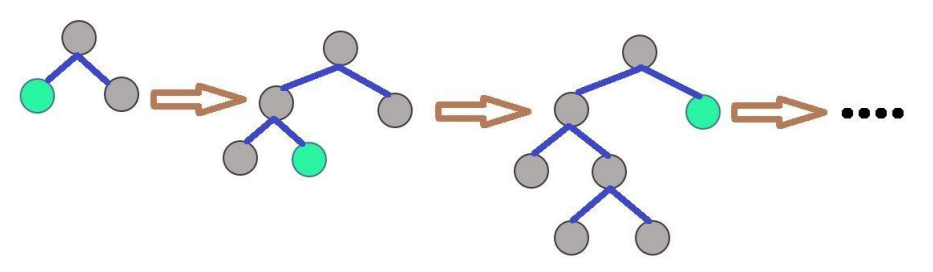
\includegraphics[width=1\textwidth]{Image/Trees Leaf-wise Growth Strategy.png}
    \caption{Chiến lược tăng trưởng theo chiều lá của cây (Trees Leaf-wise Growth Strategy)}
    \label{fig:1}
    \end{minipage}
\end{figure}
Chúng ta có thể xem quá trình học của thuật toán GTB như minh họa trong hình trên. Cây học sẽ được xây dựng số cây mục tiêu ngược trước. Cuối cùng thì giá trị ước lượng sẽ là $\sum f_n(x)$. Mô hình cuối cùng sẽ có dạng:
\[
f(x) = \sum_{i=1}^{M} (\beta_i h_i (x; \Theta_i)) = f_{M-1}(x) + \rho_M \beta_M h_M (x; \Theta_M),
\]
% Trong đó $x$ là mẫu và hàm $h(x; \Theta_i)$ là cây ra quyết định thứ $i$. Các tham số khác được tính như sau:
% \[
% \theta_M, \beta_M = \argmin_{\theta, \beta} \sum_{j=1}^{N} \left\| \frac{\partial L \left( f_{M-1}(x_j), y_j \right)}{\partial f_{M-1}(x_j)} - \beta h \left( x_j; \theta \right) \right\|^2
% \]

% \[
% \rho_M = \argmin_{\rho} \sum_{j=1}^{N} L \left( f_{M-1}(x_j) + \rho h \left( x_j; \theta_M \right), y_j \right)
% \]
\subsection{RESCNN}
Phương pháp ResCNN (Residual Convolutional Neural Network) kết hợp hai thành phần chính từ hai mô hình khác nhau: ResNet (Residual Network) và CNN (Convolutional Neural Network). Đây là một kiến trúc mạng nơ-ron sử dụng cấu trúc khối residual và các lớp tích chập để giải quyết các bài toán trong lĩnh vực thị giác máy tính, như nhận dạng hình ảnh, phân loại văn bản hình ảnh, và nhiều ứng dụng khác.

Mô hình ResCNN:

Đầu vào (Input): Dữ liệu hình ảnh được đưa vào mạng.

Convolutional Layers (Lớp tích chập): Mỗi lớp tích chập thực hiện phép tích chập trên đầu vào để trích xuất các đặc trưng của hình ảnh.

Residual Blocks (Khối Residual): Mỗi khối residual bao gồm một chuỗi các lớp tích chập được xếp chồng lên nhau. Đầu vào được truyền qua chuỗi này và sau đó cộng với đầu vào ban đầu. 
Công thức cho một residual block có thể được mô tả như sau: 
\[
\text{output} = \text{ReLU}(W_2 \cdot \text{ReLU}(W_1 \cdot \text{input} + b_1) + \text{input} + b_2)
\]
Trong đó:\\
        \indent\textbullet\ input là đầu vào của khối residual. \\
	\indent\textbullet\ $W_1$ và $W_2$ là các ma trận trọng số của các lớp tích chập trong khối. \\
 	\indent\textbullet\ $b_1$ và $b_2$ là các ma trận trọng số của các lớp tích chập trong khối. \\
 	\indent\textbullet\ ReLU là hàm kích hoạt ReLU (Rectified Linear Unit). \\

Pooling Layers (Lớp gộp): Các lớp gộp thường được sử dụng để giảm kích thước của không gian đặc trưng.

Fully Connected Layers (Lớp kết nối đầy đủ): Các lớp kết nối đầy đủ được sử dụng để chuyển đổi biểu diễn không gian đặc trưng thành dự đoán cuối cùng.

Output Layer (Lớp đầu ra): Lớp cuối cùng của mạng, thường sử dụng hàm kích hoạt phù hợp (ví dụ: softmax cho phân loại) để tạo ra dự đoán cuối cùng.
\subsection{FUZZY FOR PREDICT TIMES SERIES}
Dựa trên lý thuyết tập mờ, logic mờ và phép suy luận mờ của Zadeh , Song và Chissom  đưa ra định nghĩa về chuỗi thời gian mờ và phác thảo về cách mô hình hóa nó thông qua các phương trình quan hệ mờ và lập luận mờ. Điều này nhằm giải quyết các vấn đề dự báo khi dữ liệu lịch sử được biểu diễn dưới dạng các giá trị ngôn ngữ.
Trong chuỗi thời gian mờ, các giá trị được biểu diễn bằng các tập mờ được xác định trên phạm vi bài toán U, trong đó U = {$u_1$, $u_2$,...$u_n$}. Một tập mờ A có thể được biểu diễn bằng:
\[A = \frac{f_A(u_1)}{u_1} + \frac{f_A(u_2)}{u_2} + \cdots + \frac{f_A(u_n)}{u_n}\]

Trong đó, $f_A$ đề cập đến hàm thành viên của tập mờ A, $f_A$: U $\to$ [0, 1] và $f_A(u_i)$ đại diện cho mức độ thành viên của $u_i$ thuộc tập mờ A và i = 1, 2, ... n.
Definition 1: Đặt Y(t) (với t $\in$ 0, 1, ...) là phạm vi bài toán bao gồm các số thực, trên đó các tập mờ $f_i(t)$ (với i $\in$ 1, 2, ...) được xác định. Đặt F(t) là một tập hợp của các $f_i(t)$ (với i $\in$ 1, 2, ...). Khi đó, F(t) được gọi là một chuỗi thời gian mờ được xác định trên Y(t) (với t $\in$ 0, 1, ...).

Definition 2: Đặt F(t) (với t $\in$ 1, 2, ...) là một chuỗi thời gian mờ. Giả sử rằng tồn tại một mối quan hệ R(t - 1, t) giữa F(t) và F(t - 1) thỏa mãn F(t) = F(t - 1) * R(t - 1, t), trong đó F(t) và F(t - 1) là các tập mờ và là toán tử hợp thành max-min; lúc đó, R(t - 1, t) là một mối quan hệ logic mờ được biểu thị bởi F(t - 1) $\to$ F(t).

Definition 3: Giả sử F(t) phụ thuộc vào F(t - 1), F(t - 2), . . . , F(t - k), nó có thể được biểu diễn bằng một mối quan hệ logic mờ: F(t - k + 1), . . . , F(t - 1), F(t - 1) $\to$ F(t).

Mô hình Fuzzy time series sử dụng một khung khái niệm bốn bước để dự đoán: (1) xác định phạm vi bài toán và chia thành các khoảng; (2) xác định các tập mờ trên phạm vi bài toán và làm mờ chuỗi thời gian; (3) xây dựng mô hình của các mối quan hệ logic mờ hiện có trong chuỗi thời gian đã được làm mờ; và (4) dự đoán và giải mã các giá trị dự đoán.
\section{THỰC NGHIỆM}
\subsection{THỰC NGHIỆM TRÊN BỘ BA DỮ LIỆU}
\subsubsection{ARIMA}
\begin{figure}[H]
    \centering
    \begin{minipage}{0.5\textwidth}
    \centering
    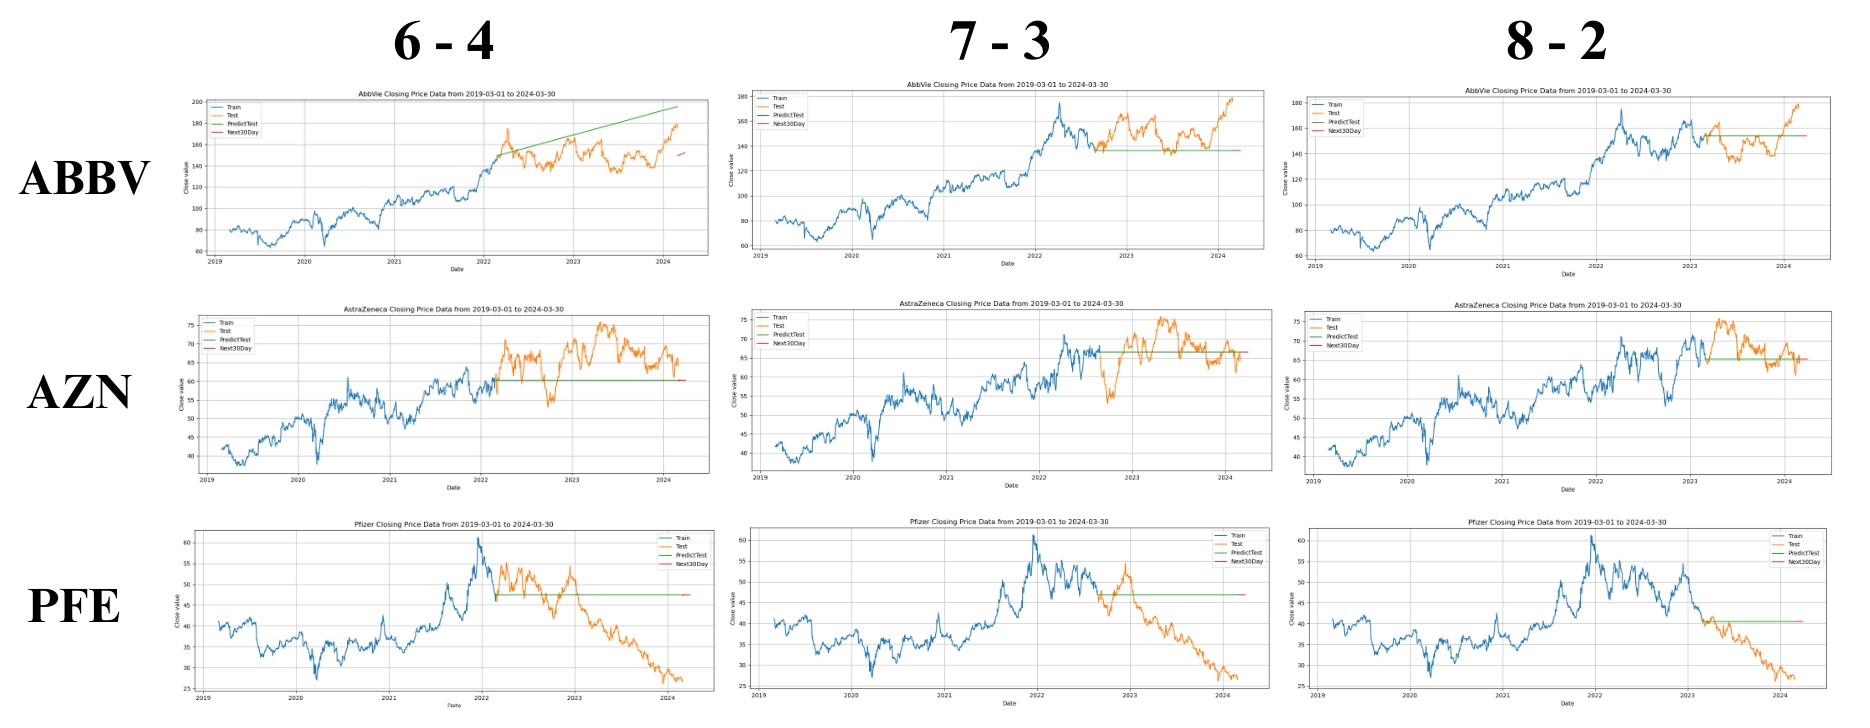
\includegraphics[width=1\textwidth]{Image/ARIMA30.png}
    \caption{Kết quả thực nghiệm ARIMA - 30 ngày}
    \label{fig:arima30}
    \end{minipage}
\end{figure}
\vspace{-15pt}
\begin{figure}[H]
    \centering
    \begin{minipage}{0.5\textwidth}
    \centering
    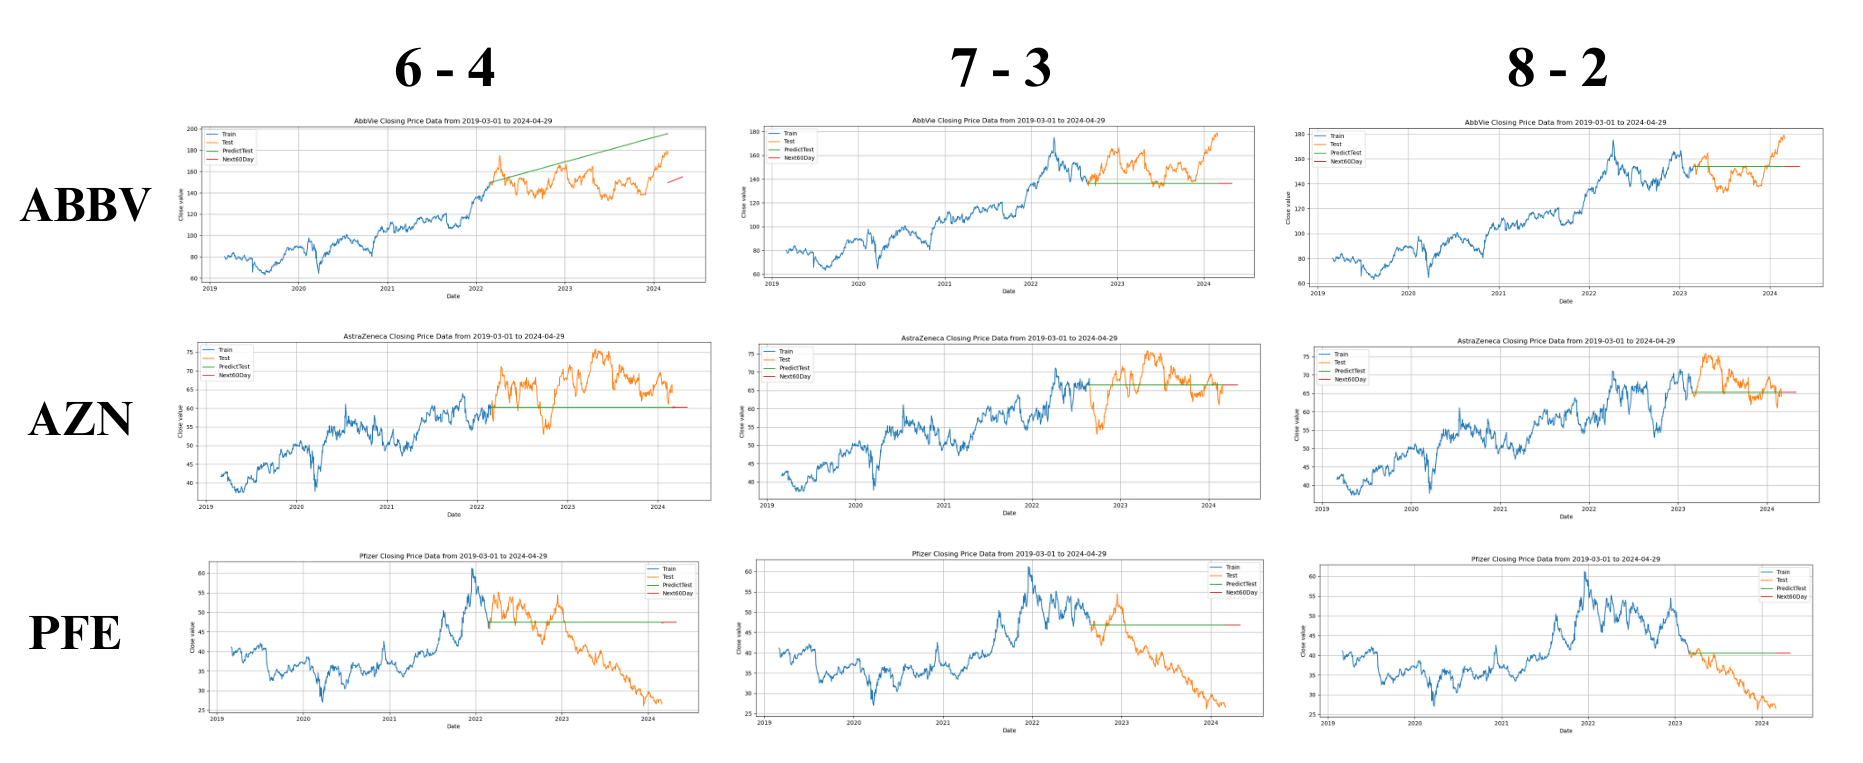
\includegraphics[width=1\textwidth]{Image/ARIMA60.png}
    \caption{Kết quả thực nghiệm ARIMA - 60 ngày}
    \label{fig:arima60}
    \end{minipage}
\end{figure}
\vspace{-10pt}
\begin{figure}[H]
    \centering
    \begin{minipage}{0.5\textwidth}
    \centering
    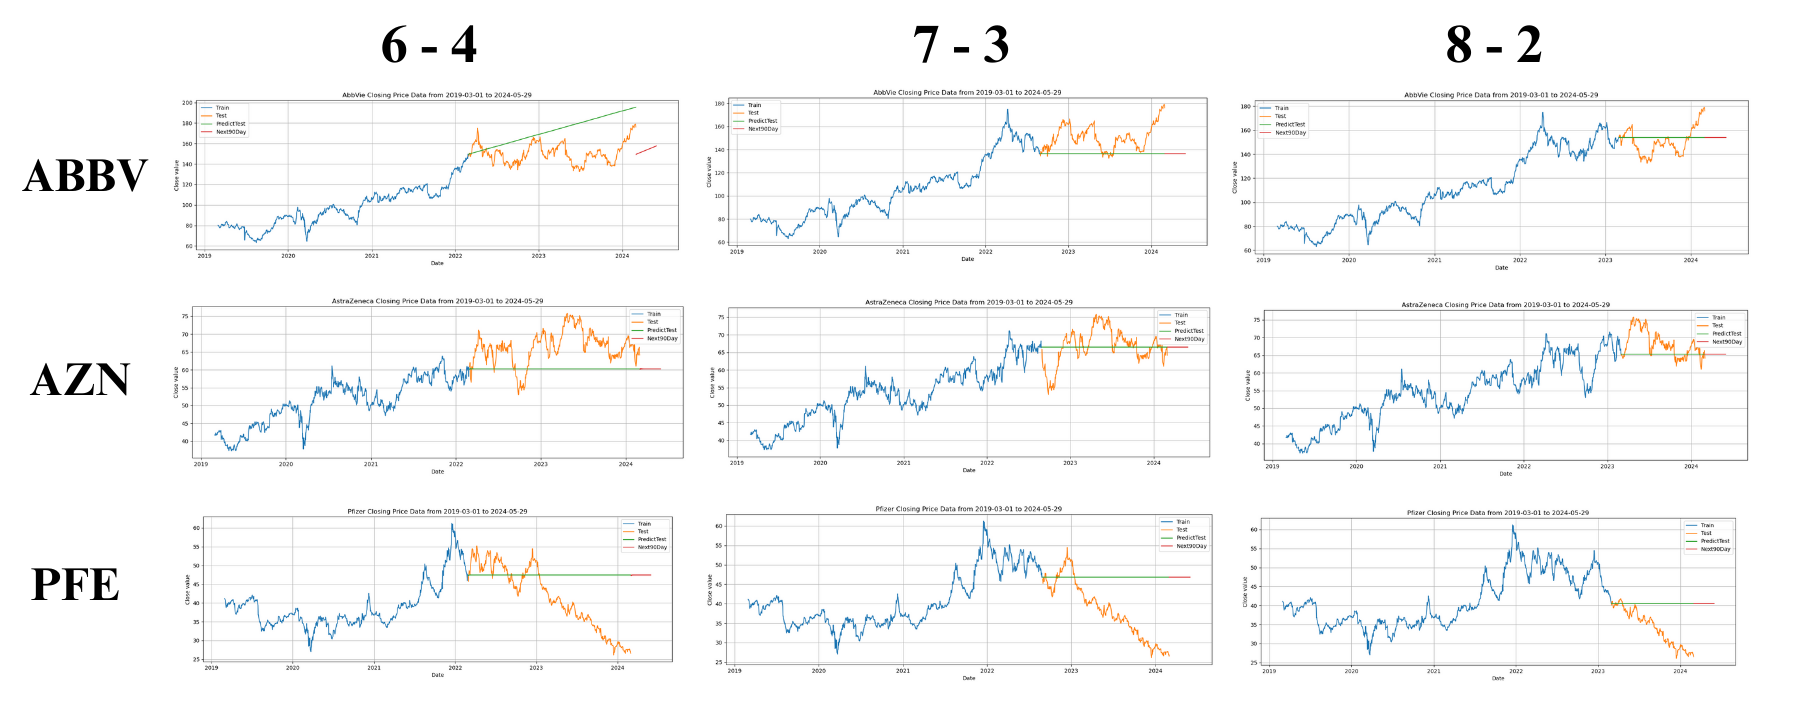
\includegraphics[width=1\textwidth]{Image/ARIMA90.png}
    \caption{Kết quả thực nghiệm ARIMA - trong 90 ngày}
    \label{fig:1}
    \end{minipage}
\end{figure}
\vspace{-20pt}
\subsubsection{GRU}
\vspace{-30pt}
\begin{figure}[H]
    \centering
    \begin{minipage}{0.5\textwidth}
    \centering
    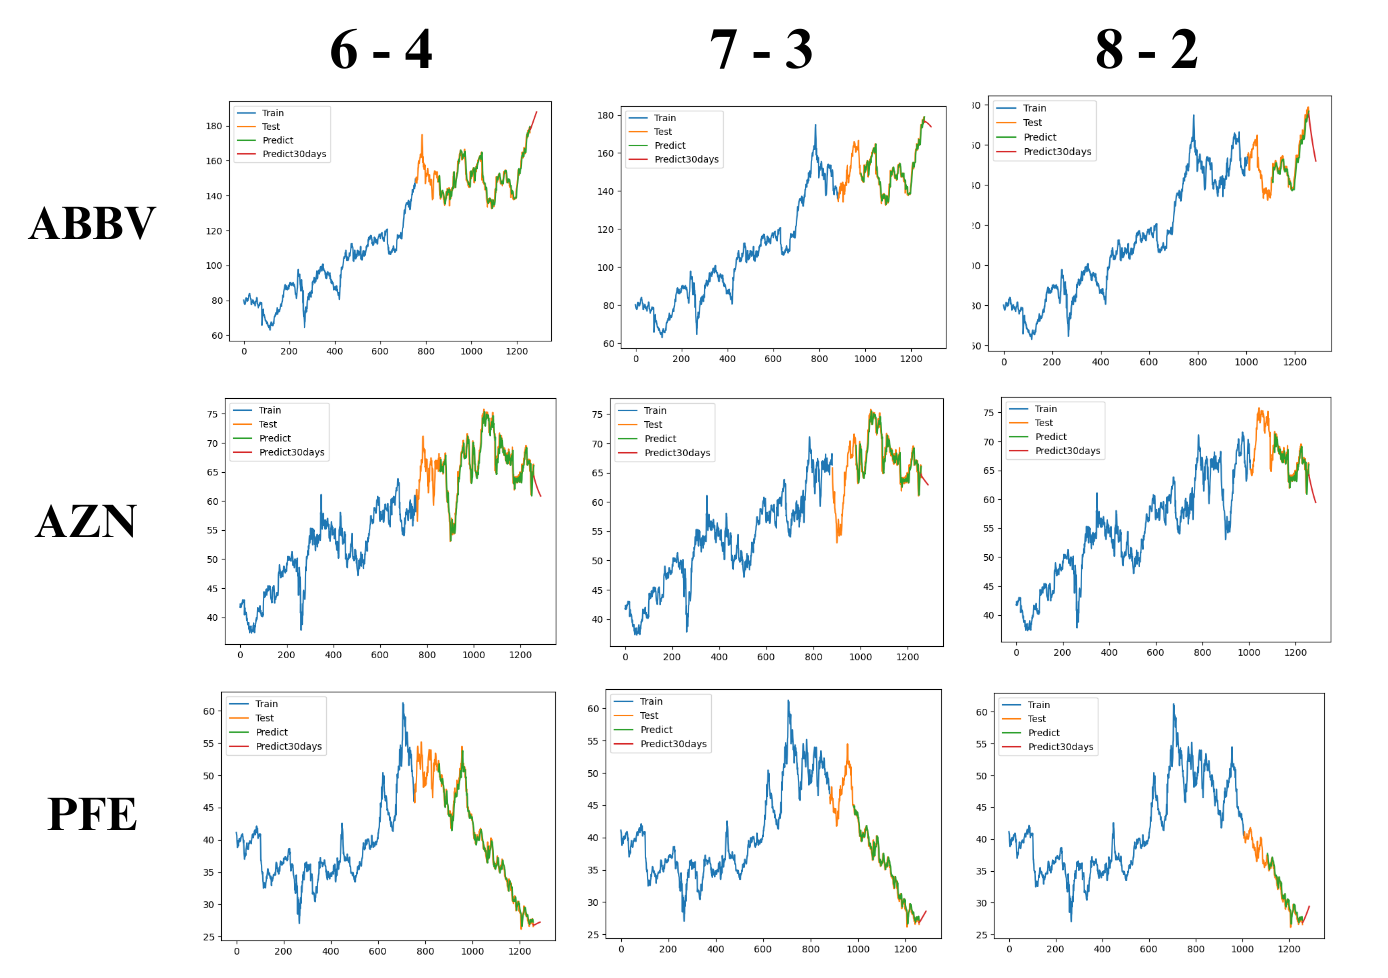
\includegraphics[width=1\textwidth]{Image/GRU30.png}
    \caption{Kết quả thực nghiệm GRU - 30 ngày}
    \label{fig:1}
    \end{minipage}
\end{figure}
\vspace{-40pt}
\begin{figure}[H]
    \centering
    \begin{minipage}{0.5\textwidth}
    \centering
    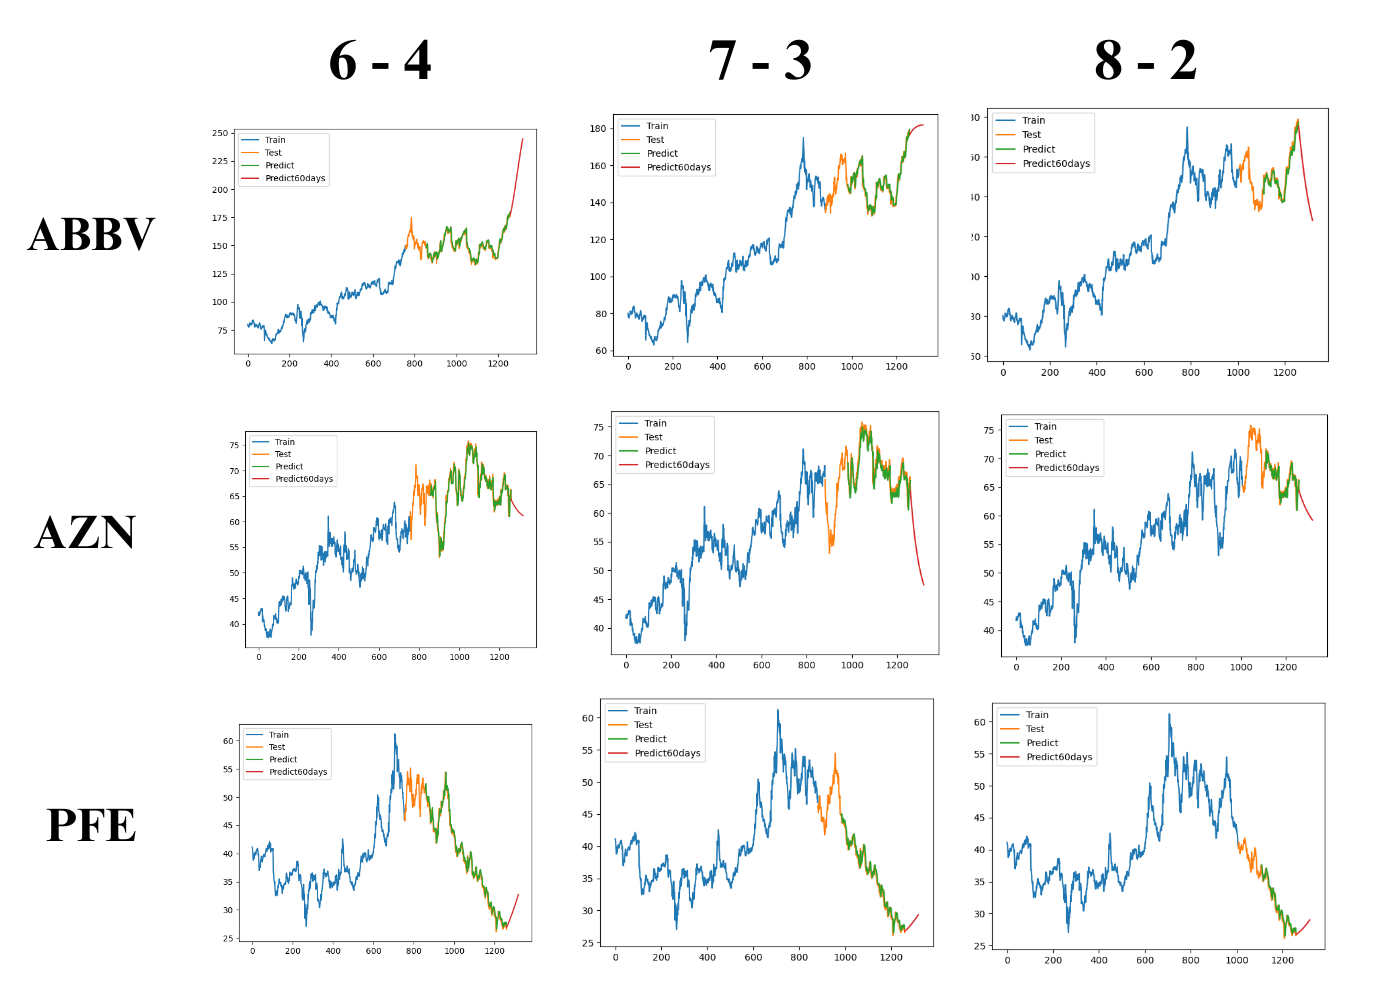
\includegraphics[width=1\textwidth]{Image/GRU60.png}
    \caption{Kết quả thực nghiệm GRU - 60 ngày}
    \label{fig:1}
    \end{minipage}
\end{figure}
\vspace{-20pt}
\begin{figure}[H]
    \centering
    \begin{minipage}{0.5\textwidth}
    \centering
    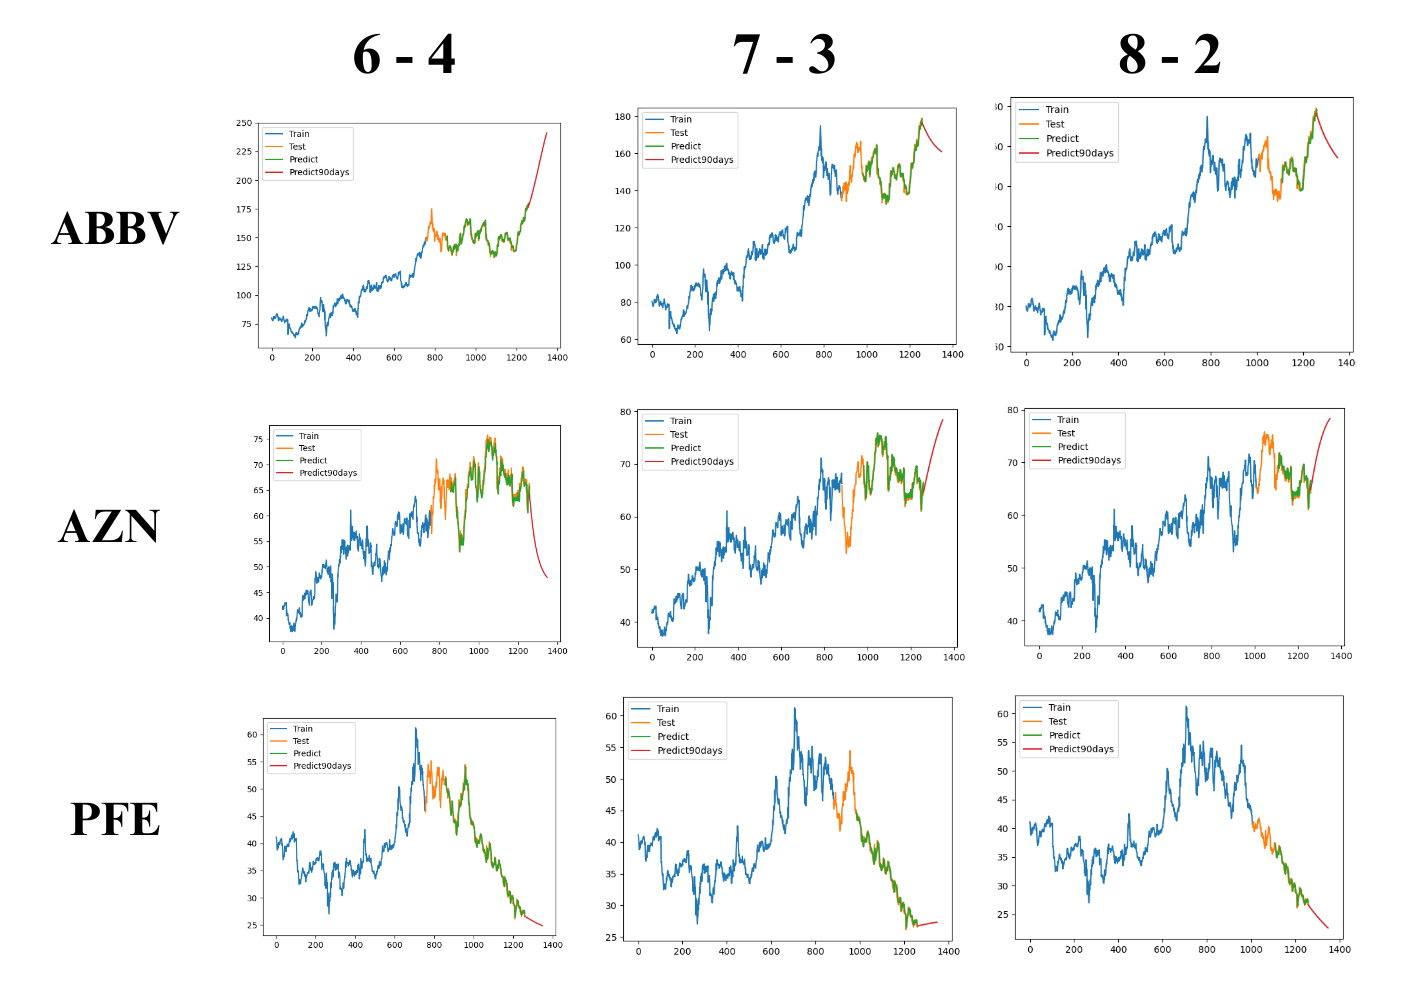
\includegraphics[width=1\textwidth]{Image/GRU90.png}
    \caption{Kết quả thực nghiệm GRU - 90 ngày}
    \label{fig:1}
    \end{minipage}
\end{figure}
\subsubsection{LINEAR REGRESSION}
\vspace{-15pt}
\begin{figure}[H]
    \centering
    \begin{minipage}{0.5\textwidth}
    \centering
    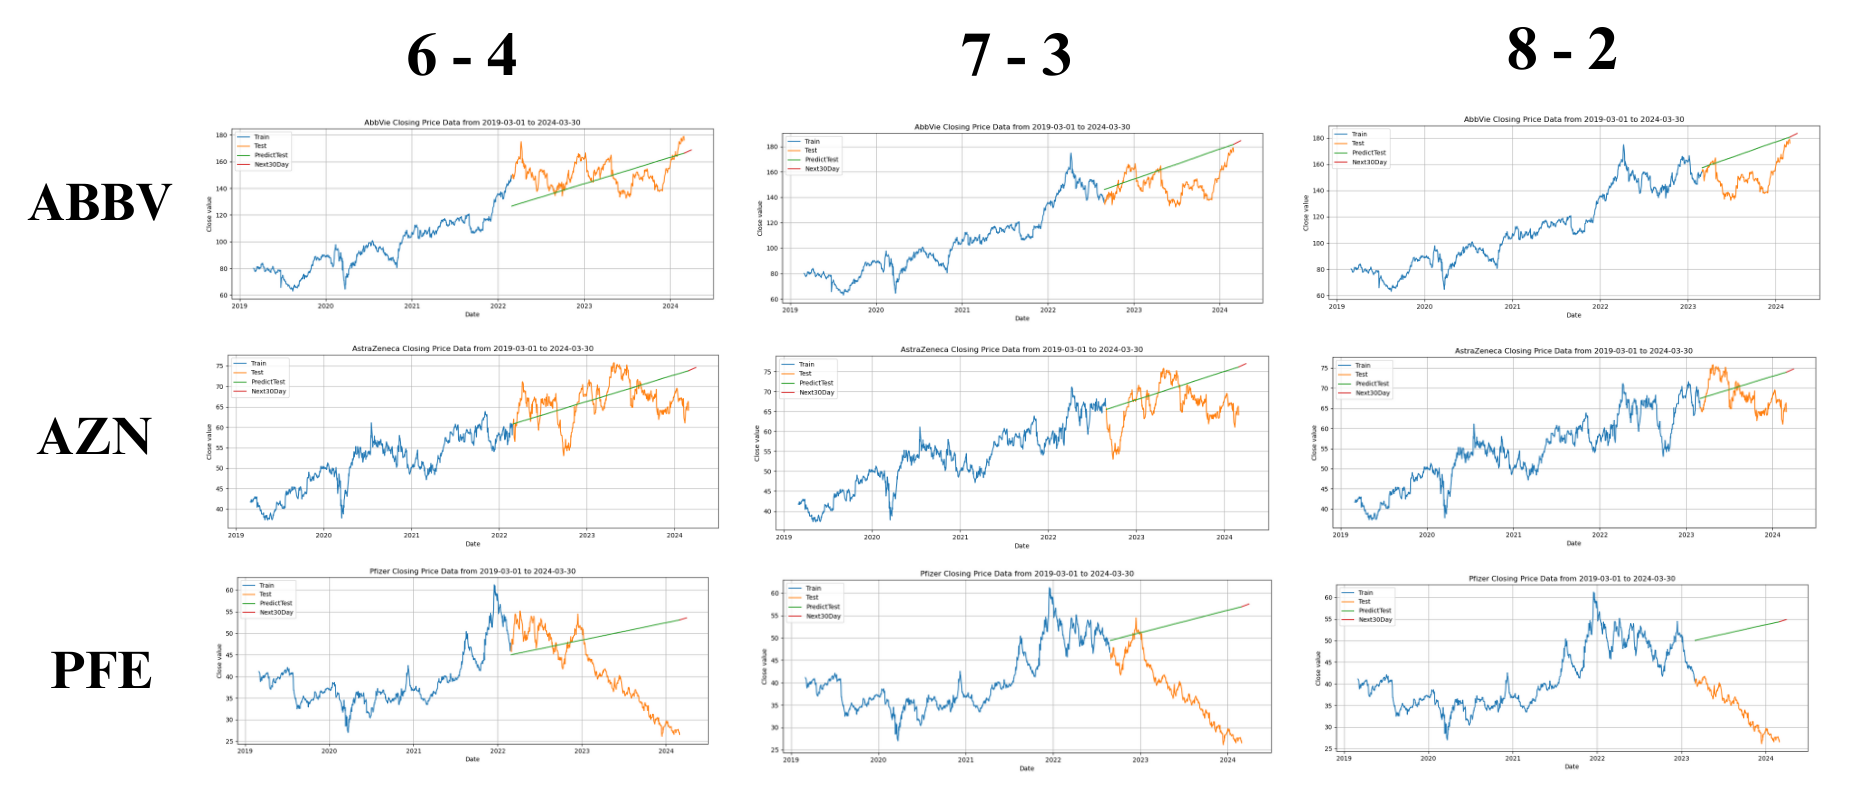
\includegraphics[width=1\textwidth]{Image/LR30.png}
    \caption{Kết quả thực nghiệm LINEAR REGRESSION -30 ngày}
    \label{fig:1}
    \end{minipage}
\end{figure}
\begin{figure}[H]
    \centering
    \begin{minipage}{0.5\textwidth}
    \centering
    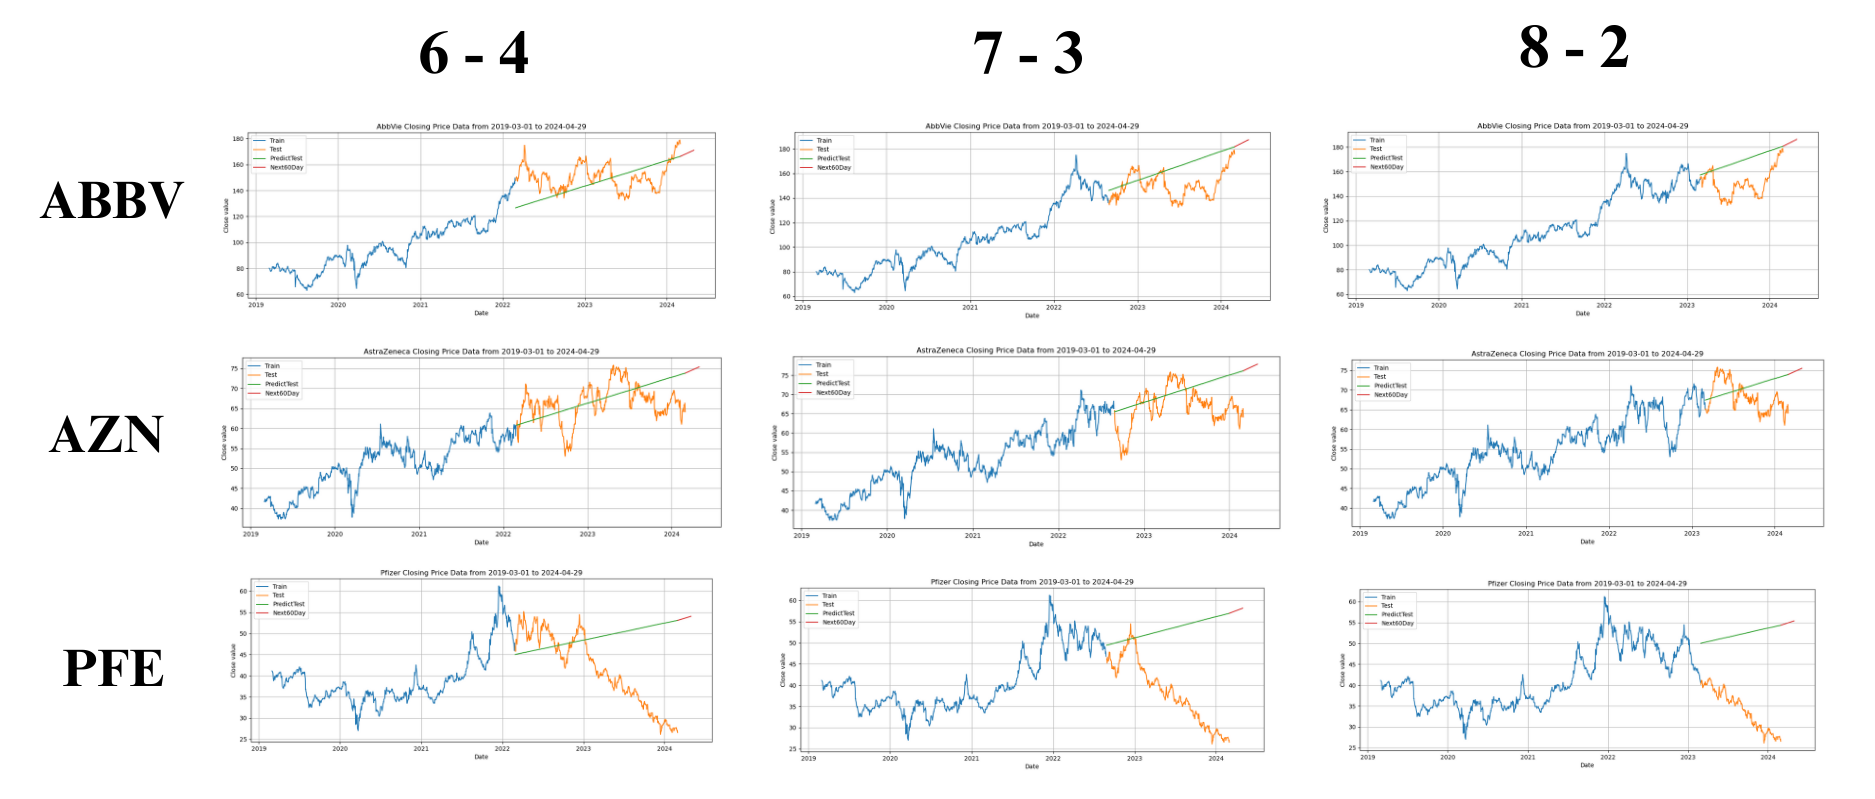
\includegraphics[width=1\textwidth]{Image/LR60.png}
    \caption{Kết quả thực nghiệm LINEAR REGRESSION - 60 ngày}
    \label{fig:1}
    \end{minipage}
\end{figure}
\begin{figure}[H]
    \centering
    \begin{minipage}{0.5\textwidth}
    \centering
    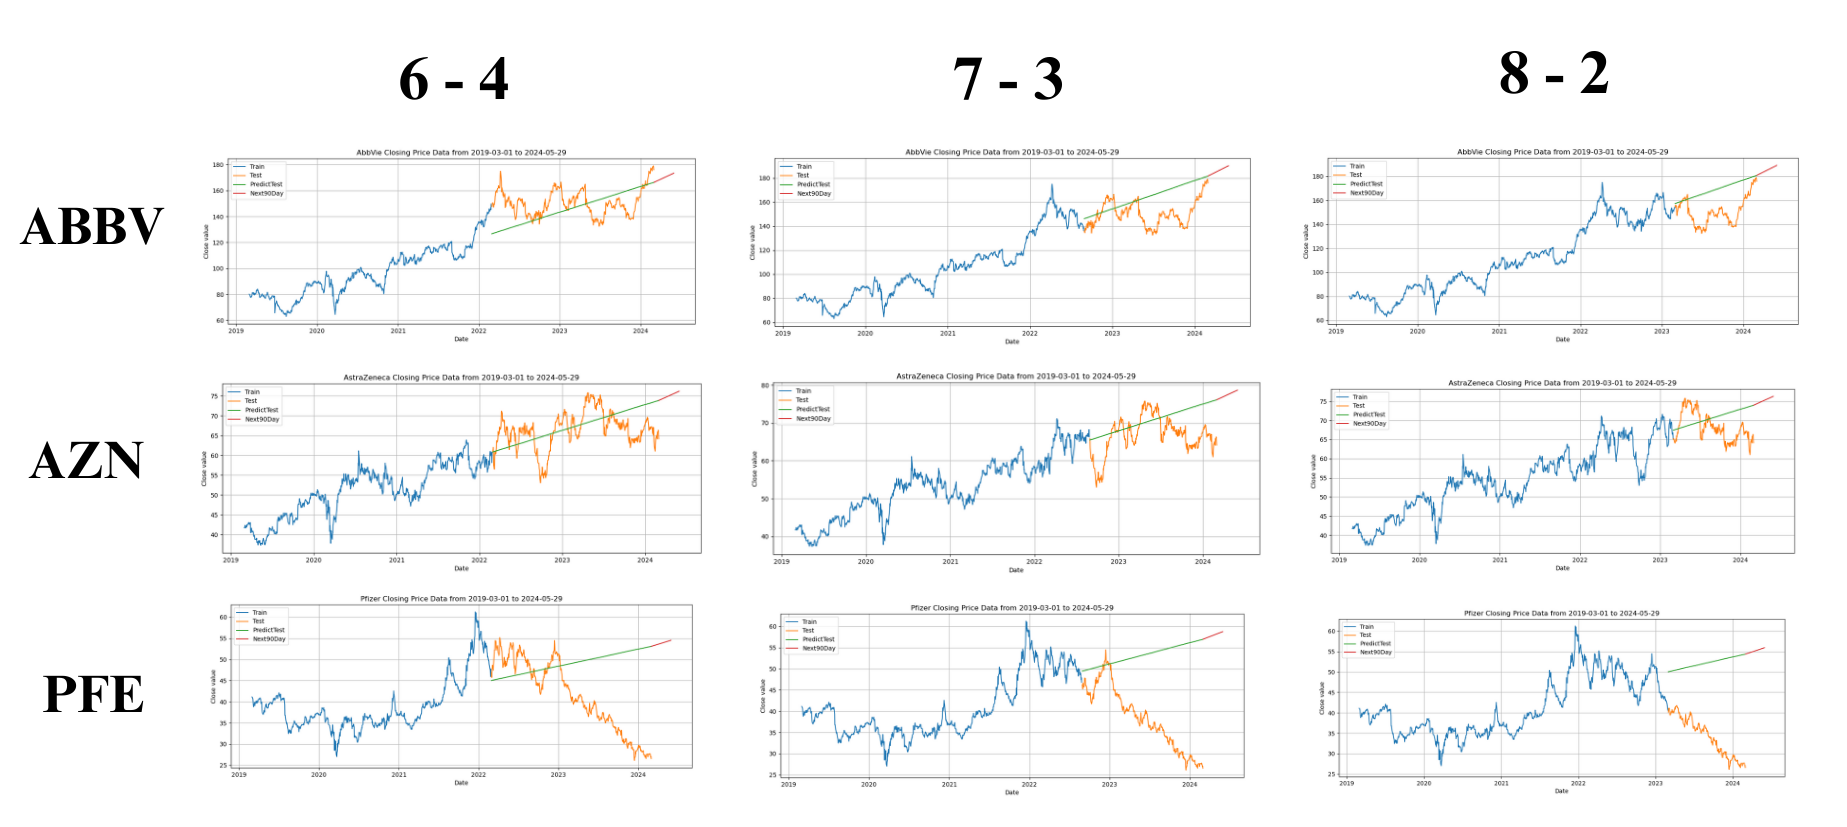
\includegraphics[width=1\textwidth]{Image/LR90.png}
    \caption{Kết quả thực nghiệm LINEAR REGRESSION - 90 ngày}
    \label{fig:1}
    \end{minipage}
\end{figure}
\subsubsection{LSTM}
\begin{figure}[H]
    \centering
    \begin{minipage}{0.5\textwidth}
    \centering
    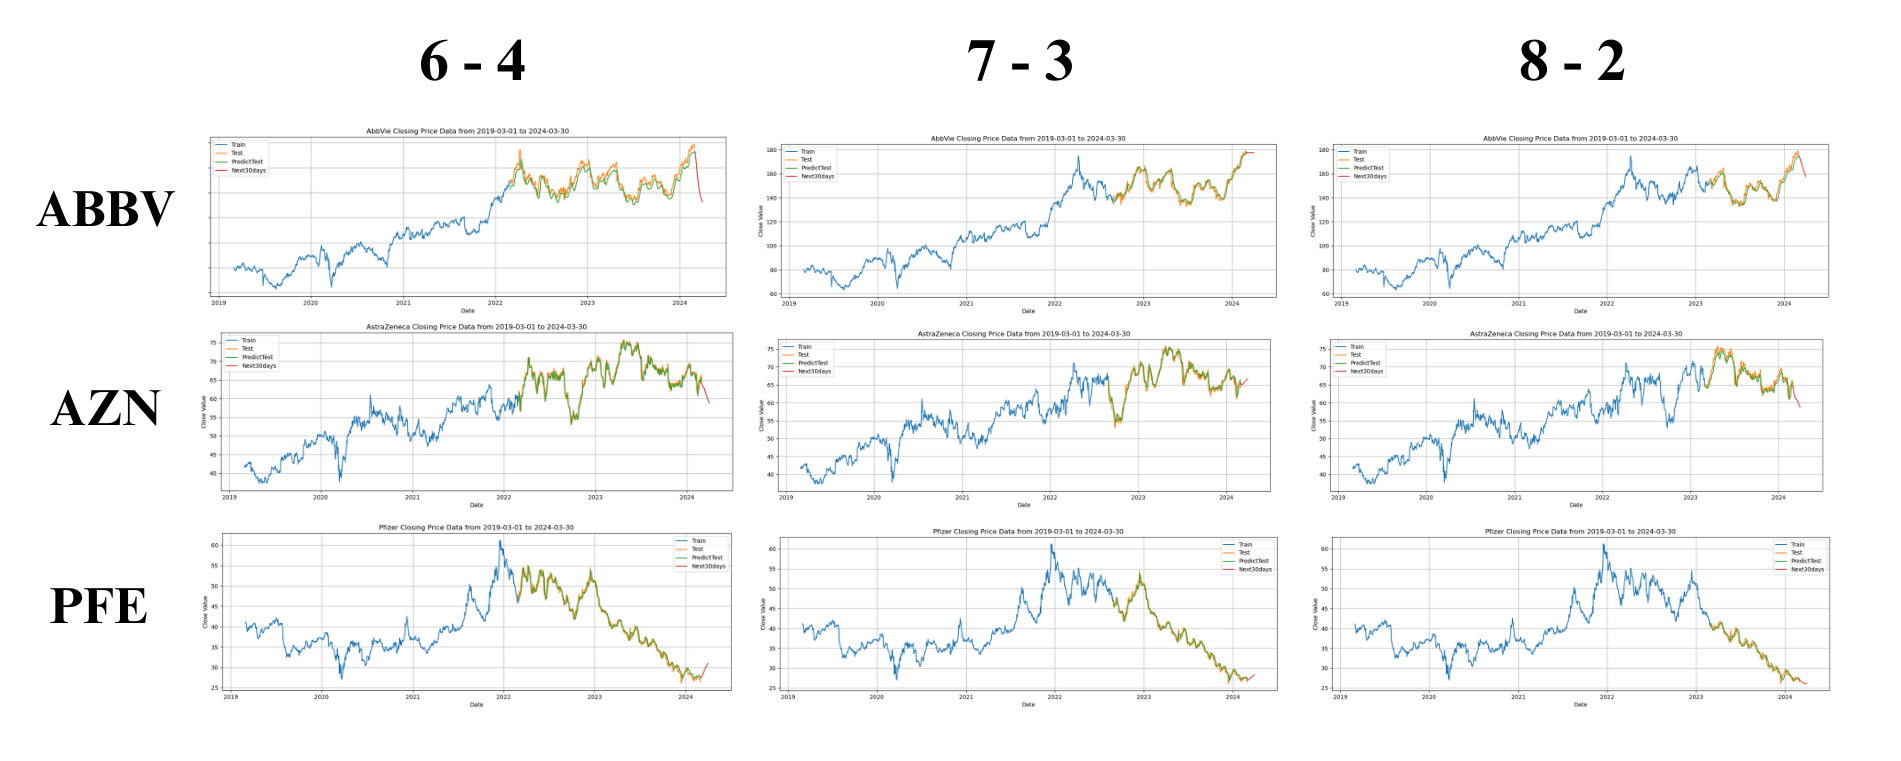
\includegraphics[width=1\textwidth]{Image/LSTM30.png}
    \caption{Kết quả thực nghiệm LSTM - 30 ngày}
    \label{fig:1}
    \end{minipage}
\end{figure}
\begin{figure}[H]
    \centering
    \begin{minipage}{0.5\textwidth}
    \centering
    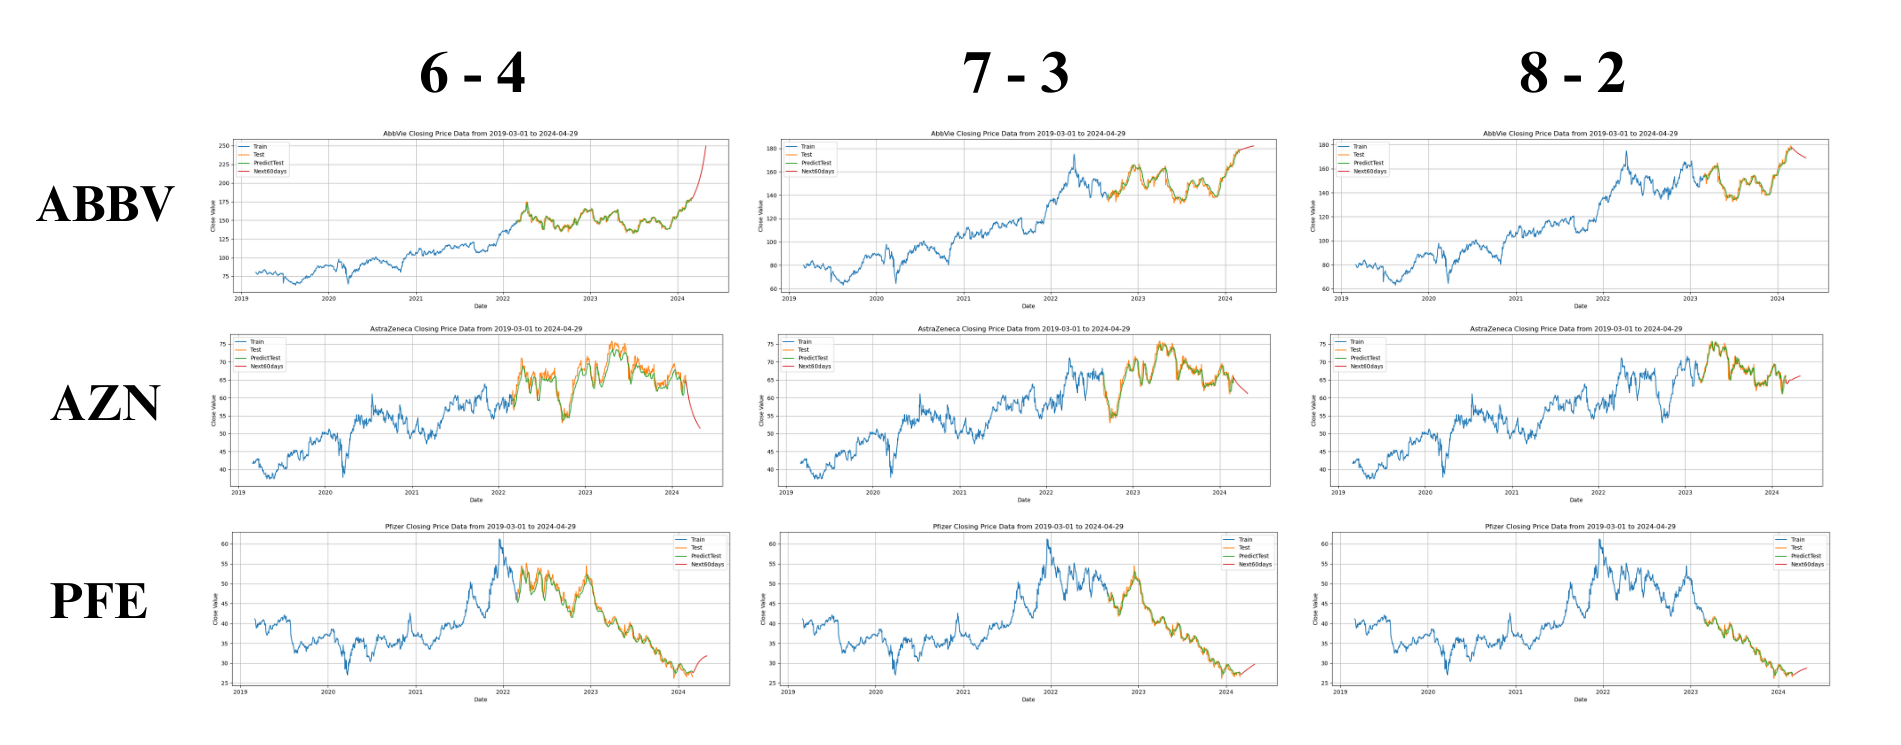
\includegraphics[width=1\textwidth]{Image/LSTM60.png}
    \caption{Kết quả thực nghiệm LSTM - 60 ngày}
    \label{fig:1}
    \end{minipage}
\end{figure}
\begin{figure}[H]
    \centering
    \begin{minipage}{0.5\textwidth}
    \centering
    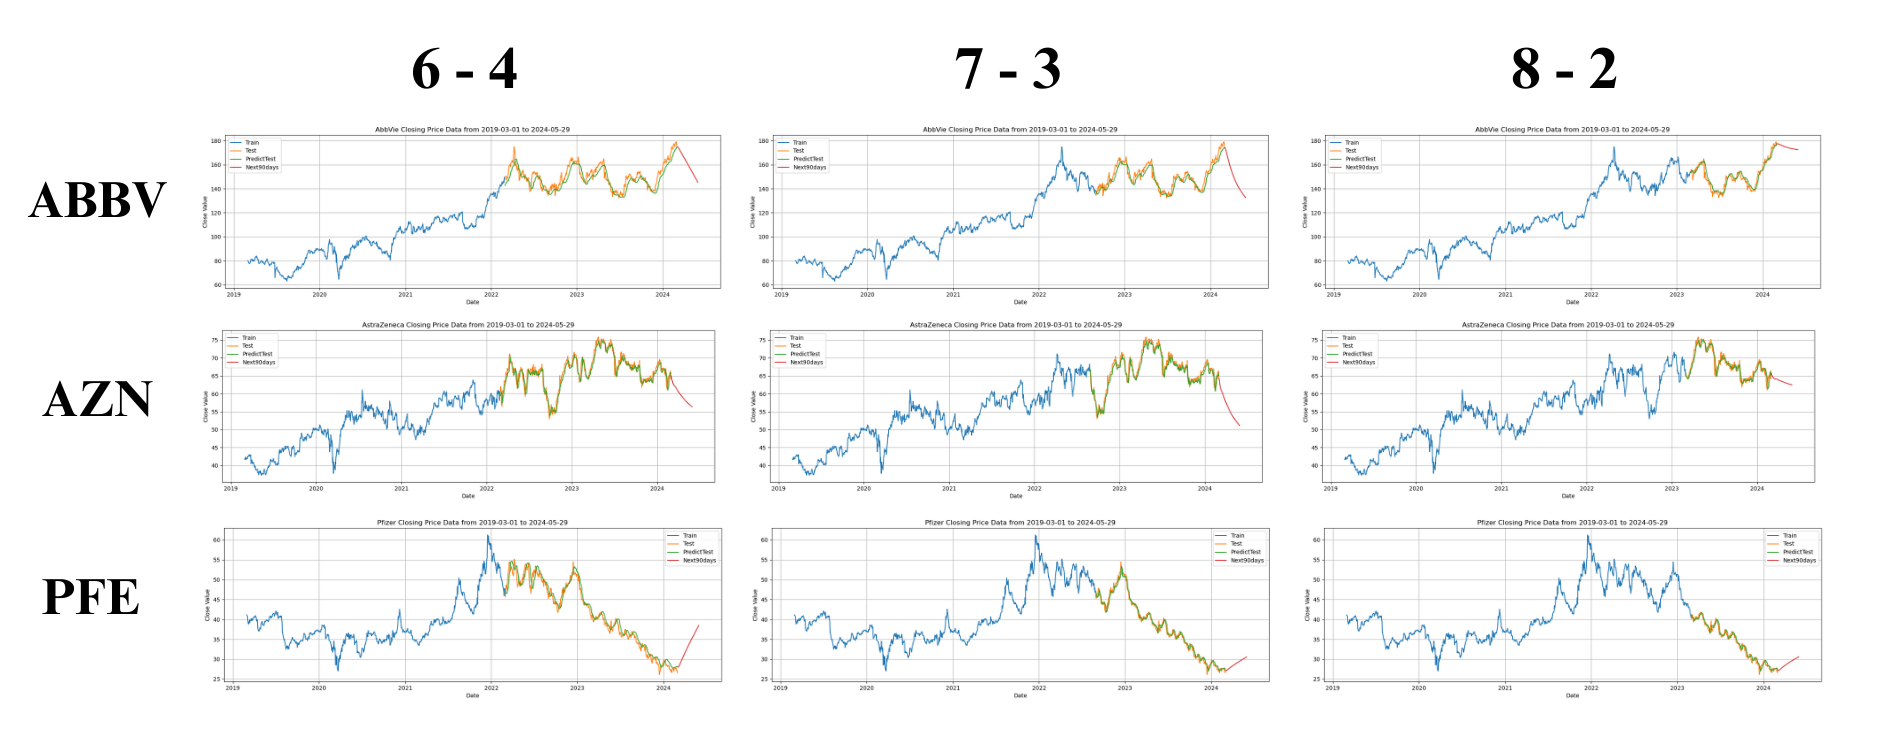
\includegraphics[width=1\textwidth]{Image/LSTM90.png}
    \caption{Kết quả thực nghiệm LSTM - 90 ngày}
    \label{fig:1}
    \end{minipage}
\end{figure}
\subsubsection{RNN}
\begin{figure}[H]
    \centering
    \begin{minipage}{0.5\textwidth}
    \centering
    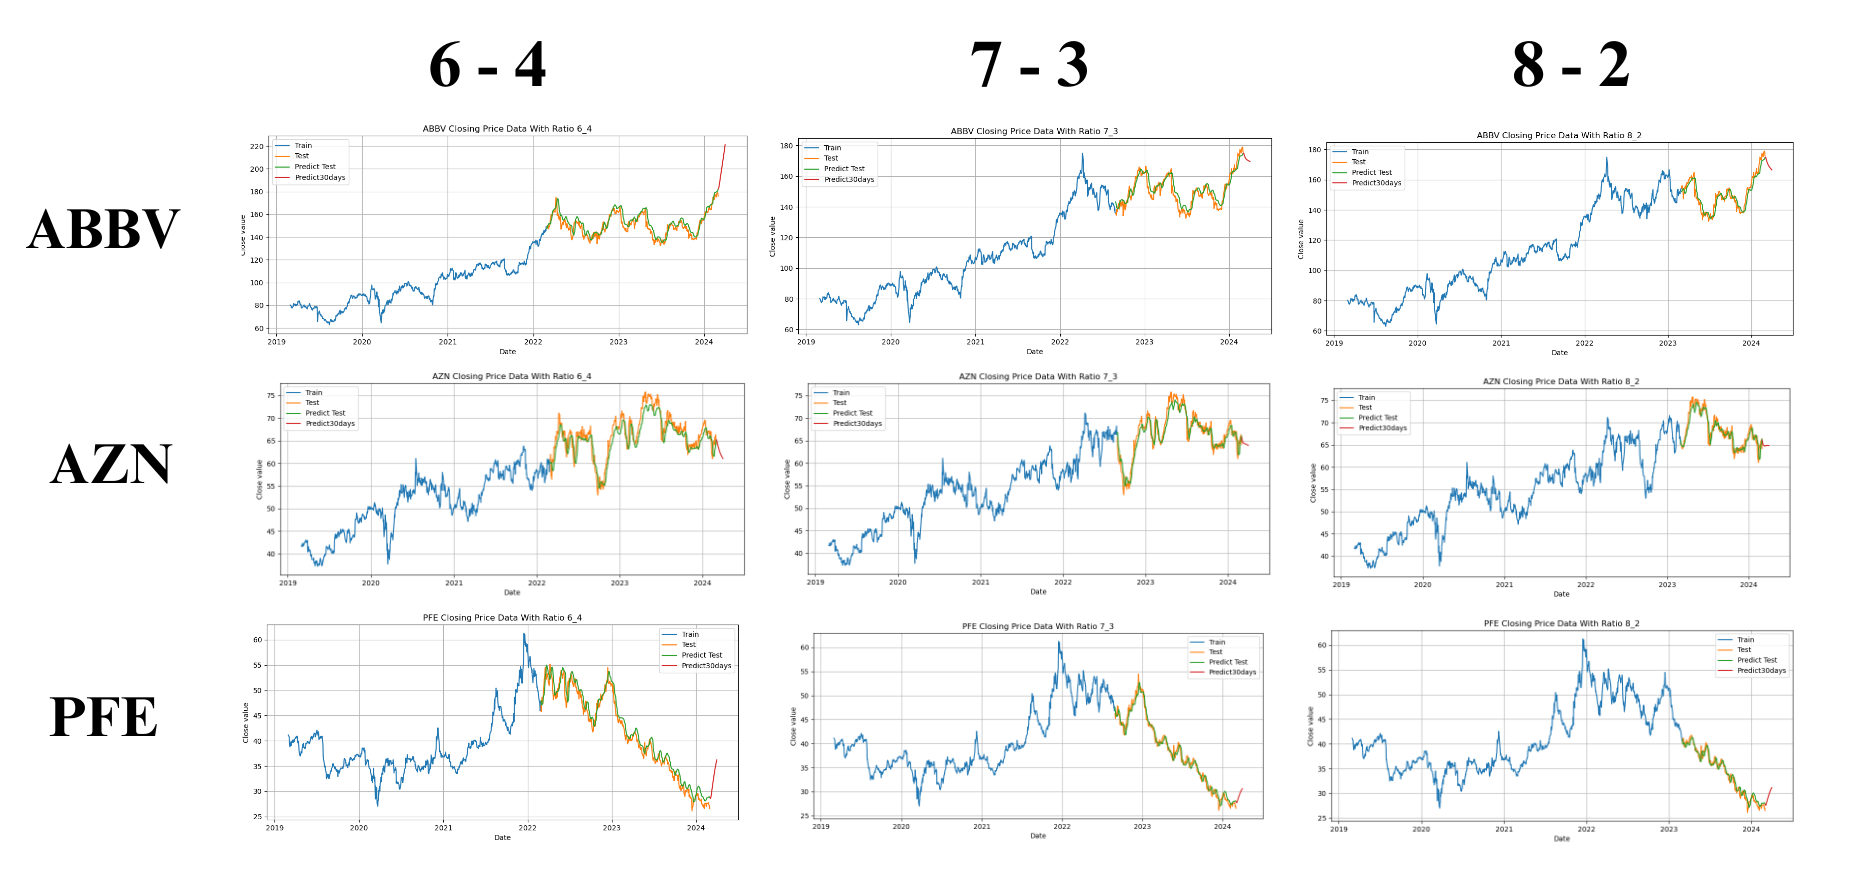
\includegraphics[width=1\textwidth]{Image/RNN30.png}
    \caption{Kết quả thực nghiệm RNN - 30 ngày}
    \label{fig:1}
    \end{minipage}
\end{figure}
\begin{figure}[H]
    \centering
    \begin{minipage}{0.5\textwidth}
    \centering
    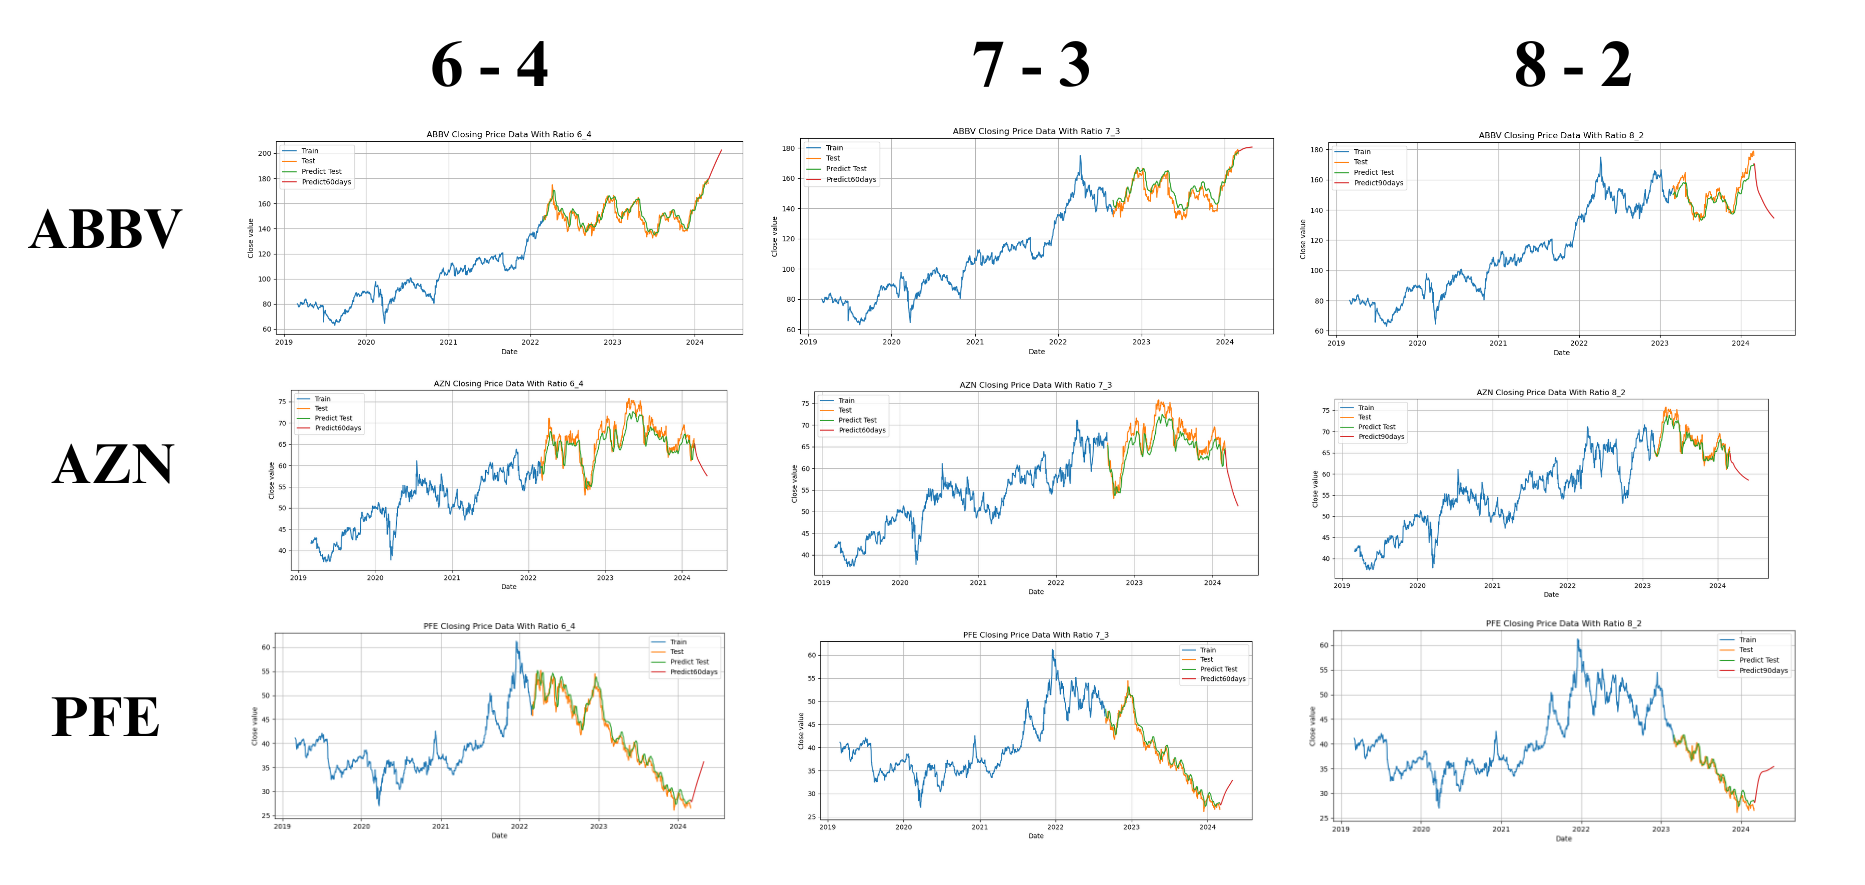
\includegraphics[width=1\textwidth]{Image/RNN60.png}
    \caption{Kết quả thực nghiệm RNN - 60 ngày}
    \label{fig:1}
    \end{minipage}
\end{figure}
\begin{figure}[H]
    \centering
    \begin{minipage}{0.5\textwidth}
    \centering
    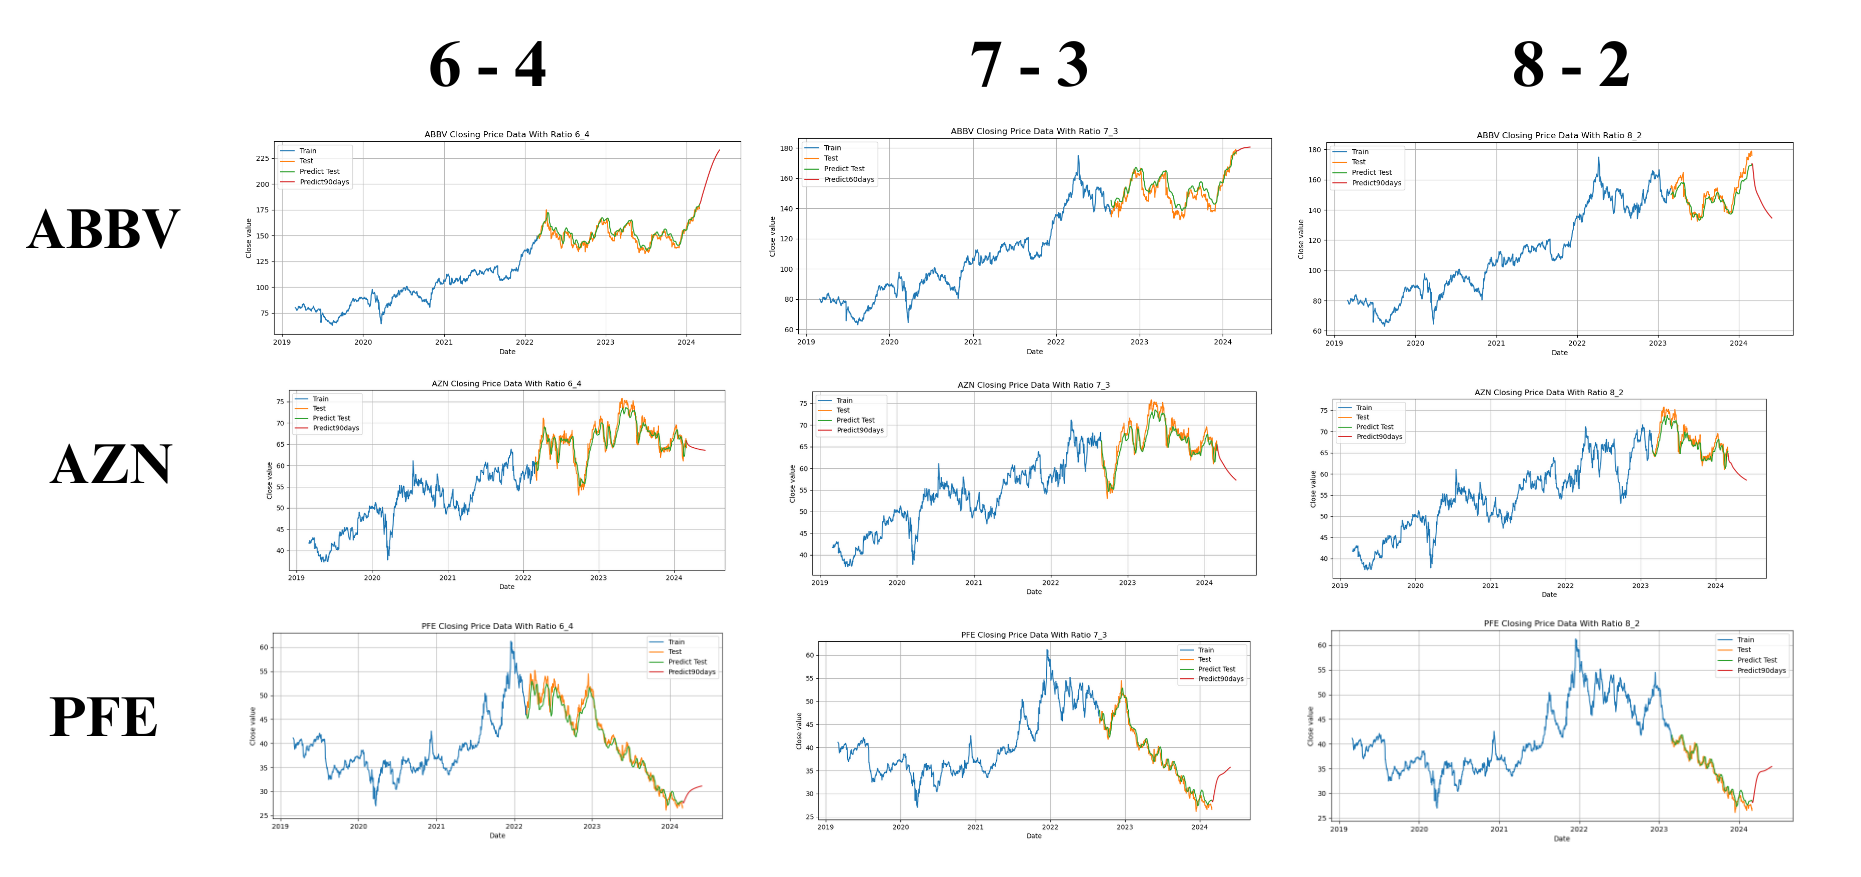
\includegraphics[width=1\textwidth]{Image/RNN90.png}
    \caption{Kết quả thực nghiệm RNN - 90 ngày}
    \label{fig:1}
    \end{minipage}
\end{figure}
\subsubsection{RANDOM FOREST}
\begin{figure}[H]
    \centering
    \begin{minipage}{0.5\textwidth}
    \centering
    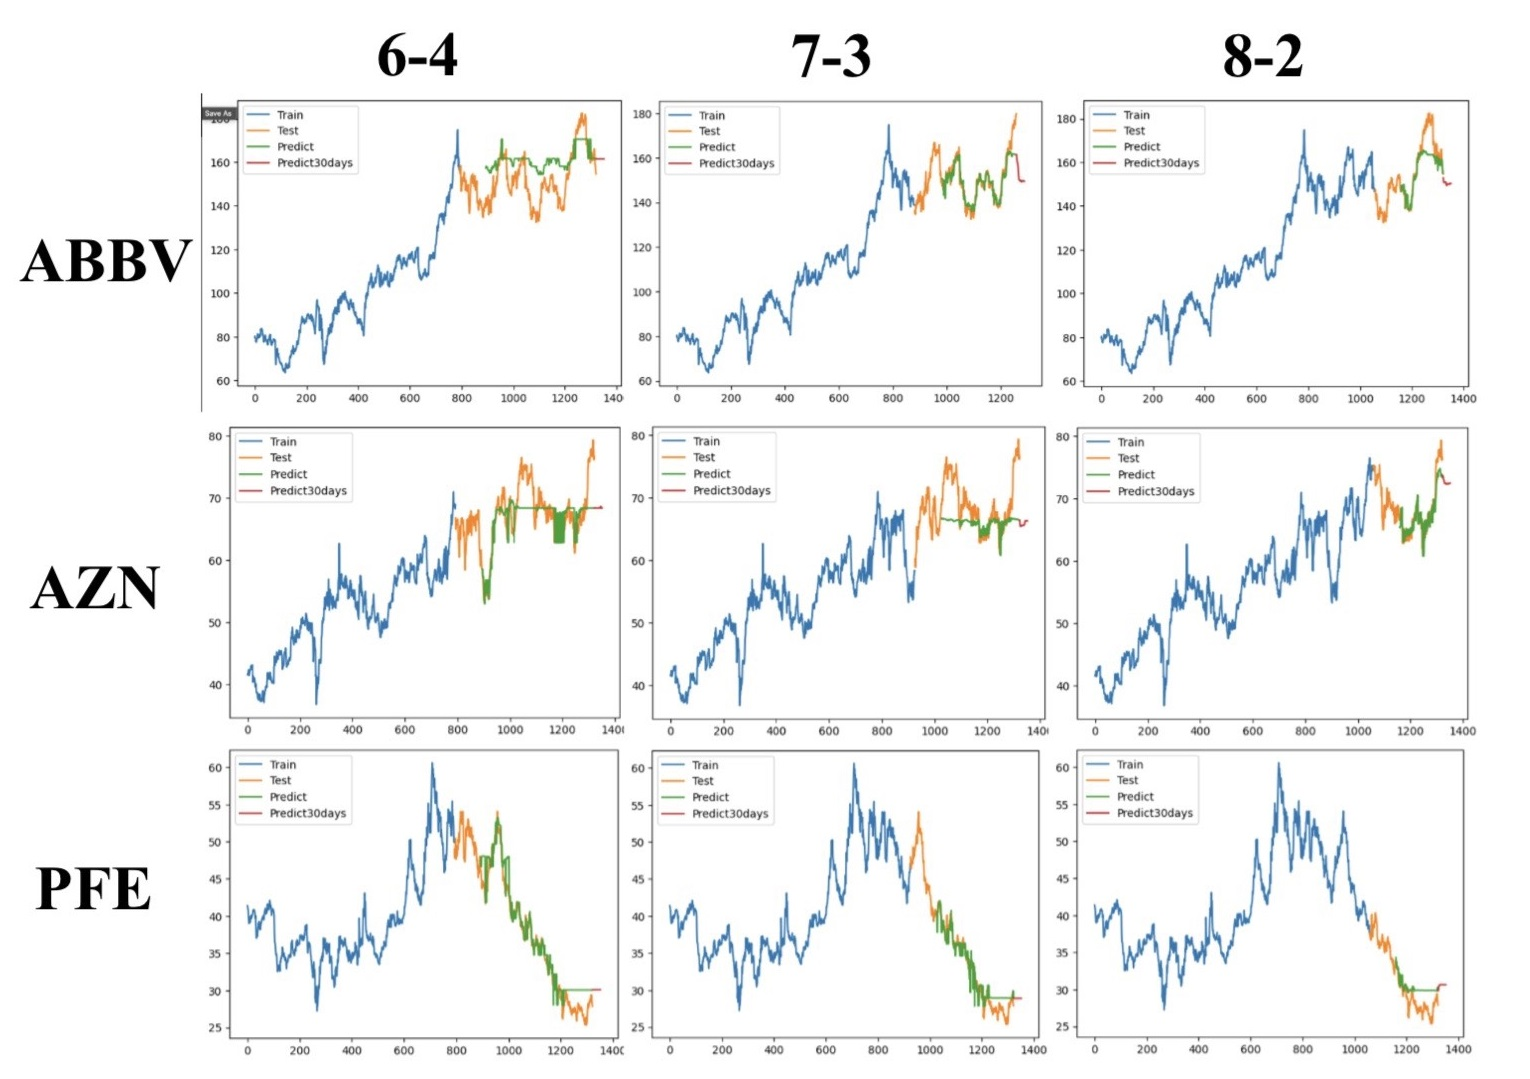
\includegraphics[width=1\textwidth]{Image/RF30.jpg}
    \caption{Kết quả thực nghiệm RANDOM FOREST - 30 ngày}
    \label{fig:1}
    \end{minipage}
\end{figure}
\begin{figure}[H]
    \centering
    \begin{minipage}{0.5\textwidth}
    \centering
    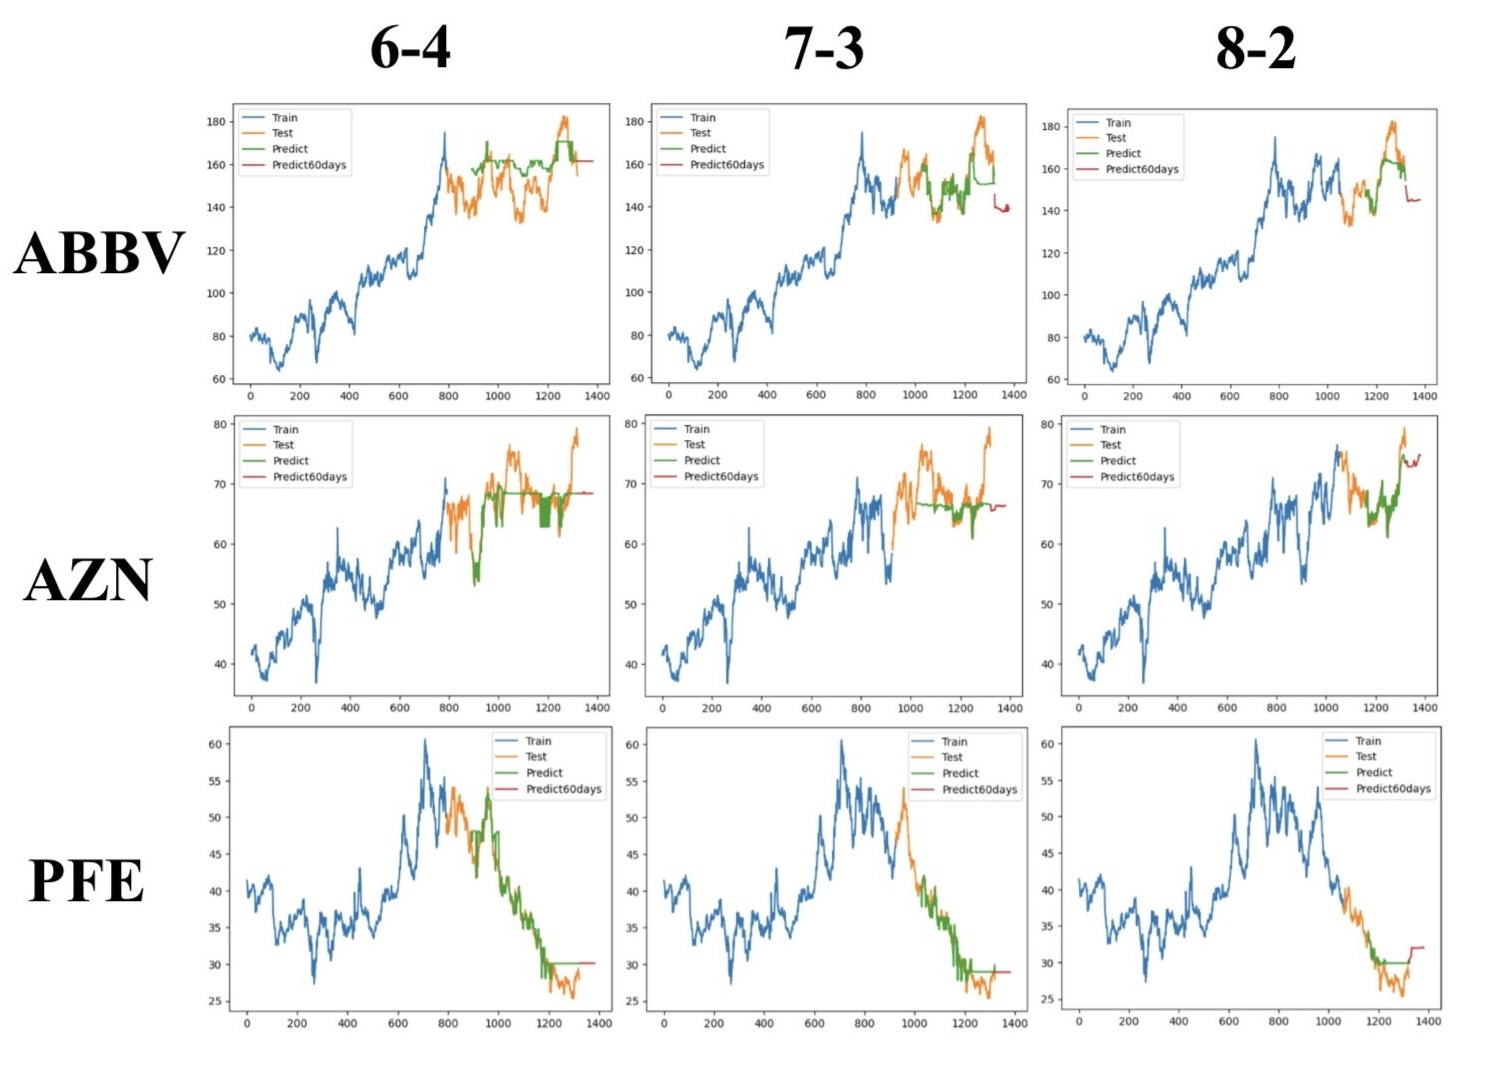
\includegraphics[width=1\textwidth]{Image/RF60.jpg}
    \caption{Kết quả thực nghiệm RANDOM FOREST - 60 ngày}
    \label{fig:1}
    \end{minipage}
\end{figure}
\begin{figure}[H]
    \centering
    \begin{minipage}{0.5\textwidth}
    \centering
    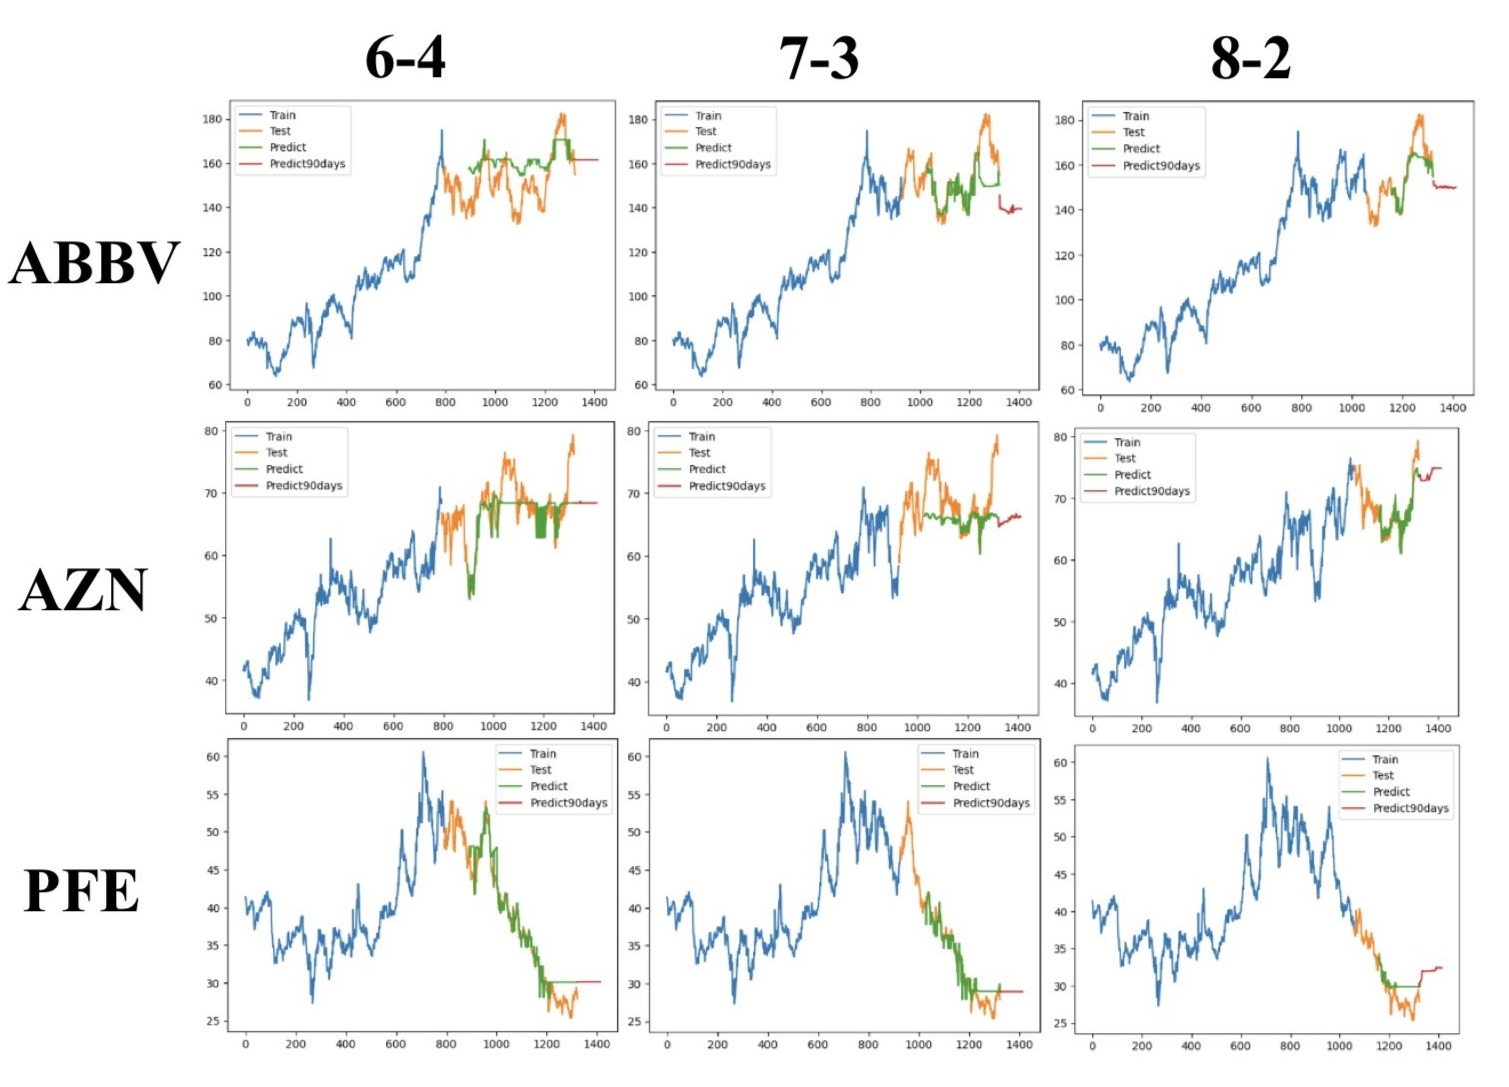
\includegraphics[width=1\textwidth]{Image/RF90.jpg}
    \caption{Kết quả thực nghiệm RANDOM FOREST - 90 ngày}
    \label{fig:1}
    \end{minipage}
\end{figure}
\subsubsection{FUZZY FOR PREDICT TIMES SERIES (FTS)}
\begin{figure}[H]
    \centering
    \begin{minipage}{0.5\textwidth}
    \centering
    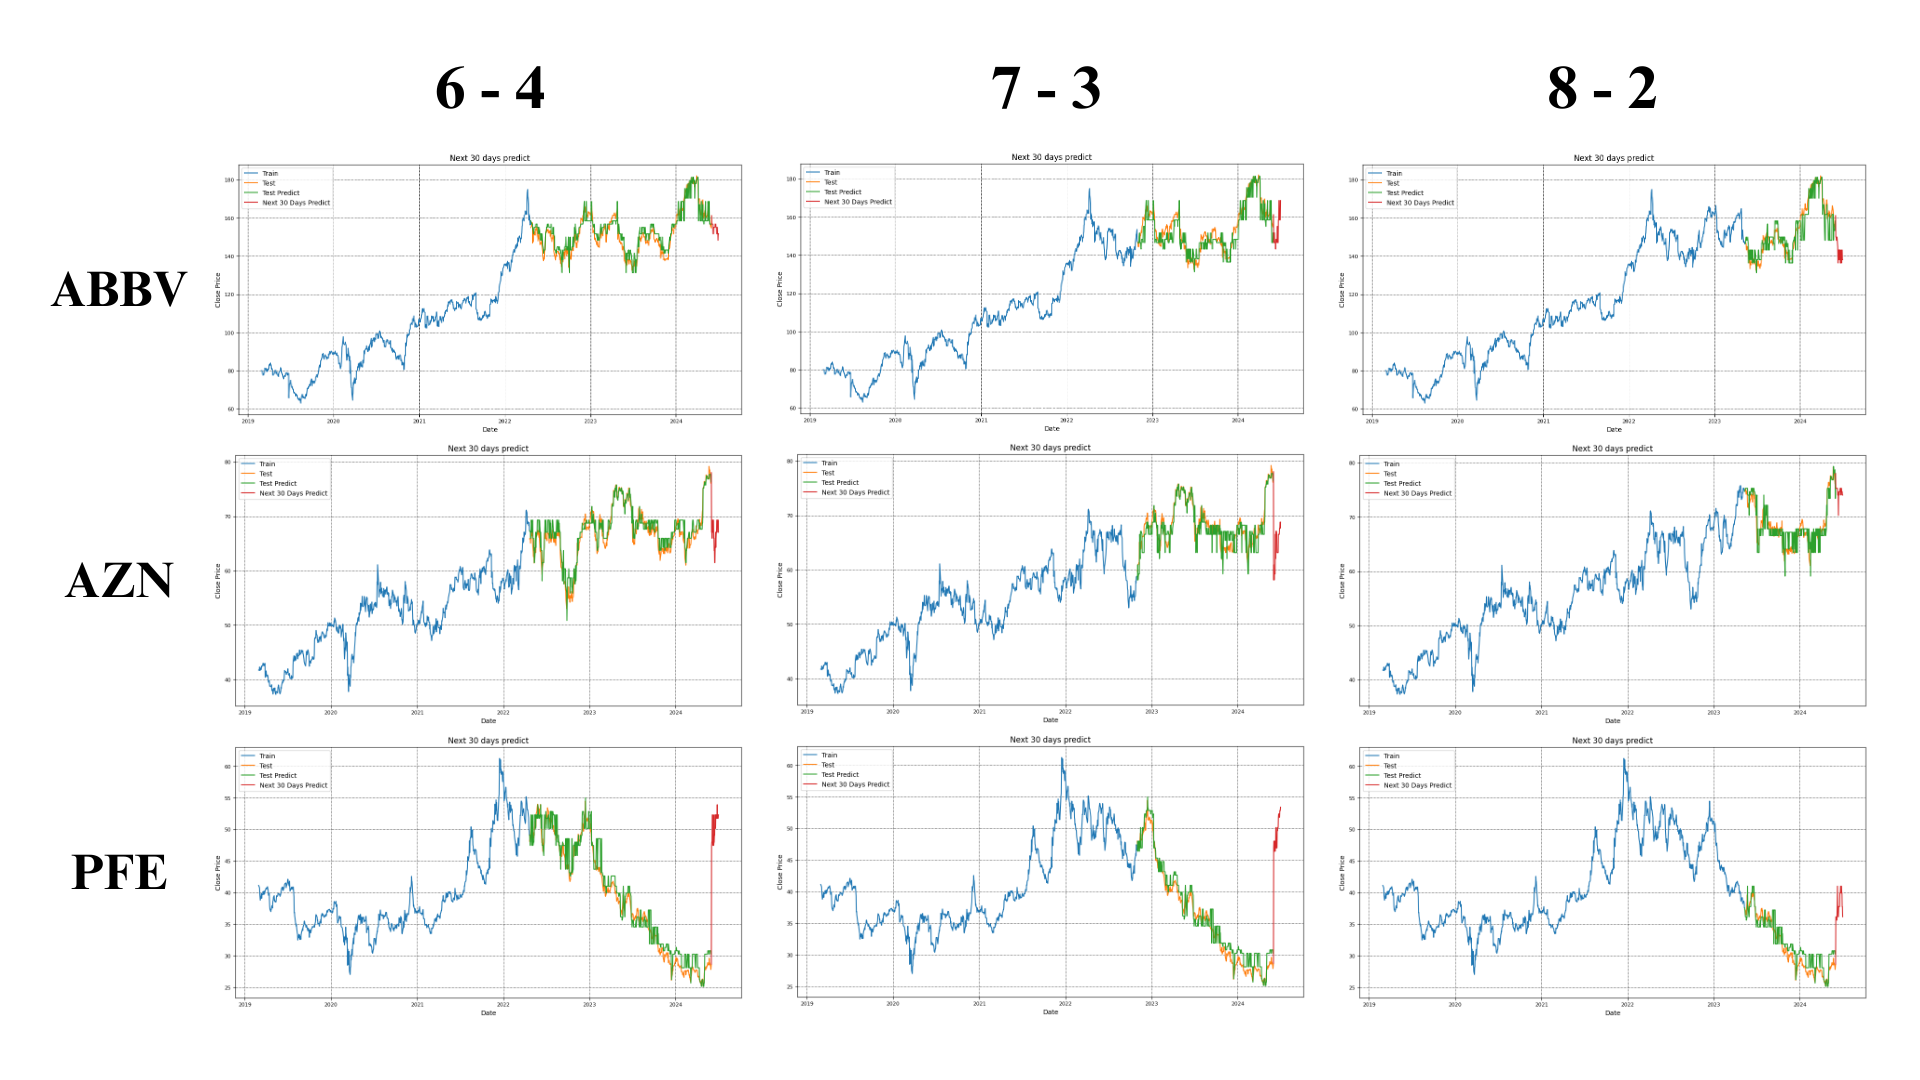
\includegraphics[width=1\textwidth]{Image/FTS30.png}
    \caption{Kết quả thực nghiệm FTS - 30 ngày}
    \label{fig:1}
    \end{minipage}
\end{figure}
\begin{figure}[H]
    \centering
    \begin{minipage}{0.5\textwidth}
    \centering
    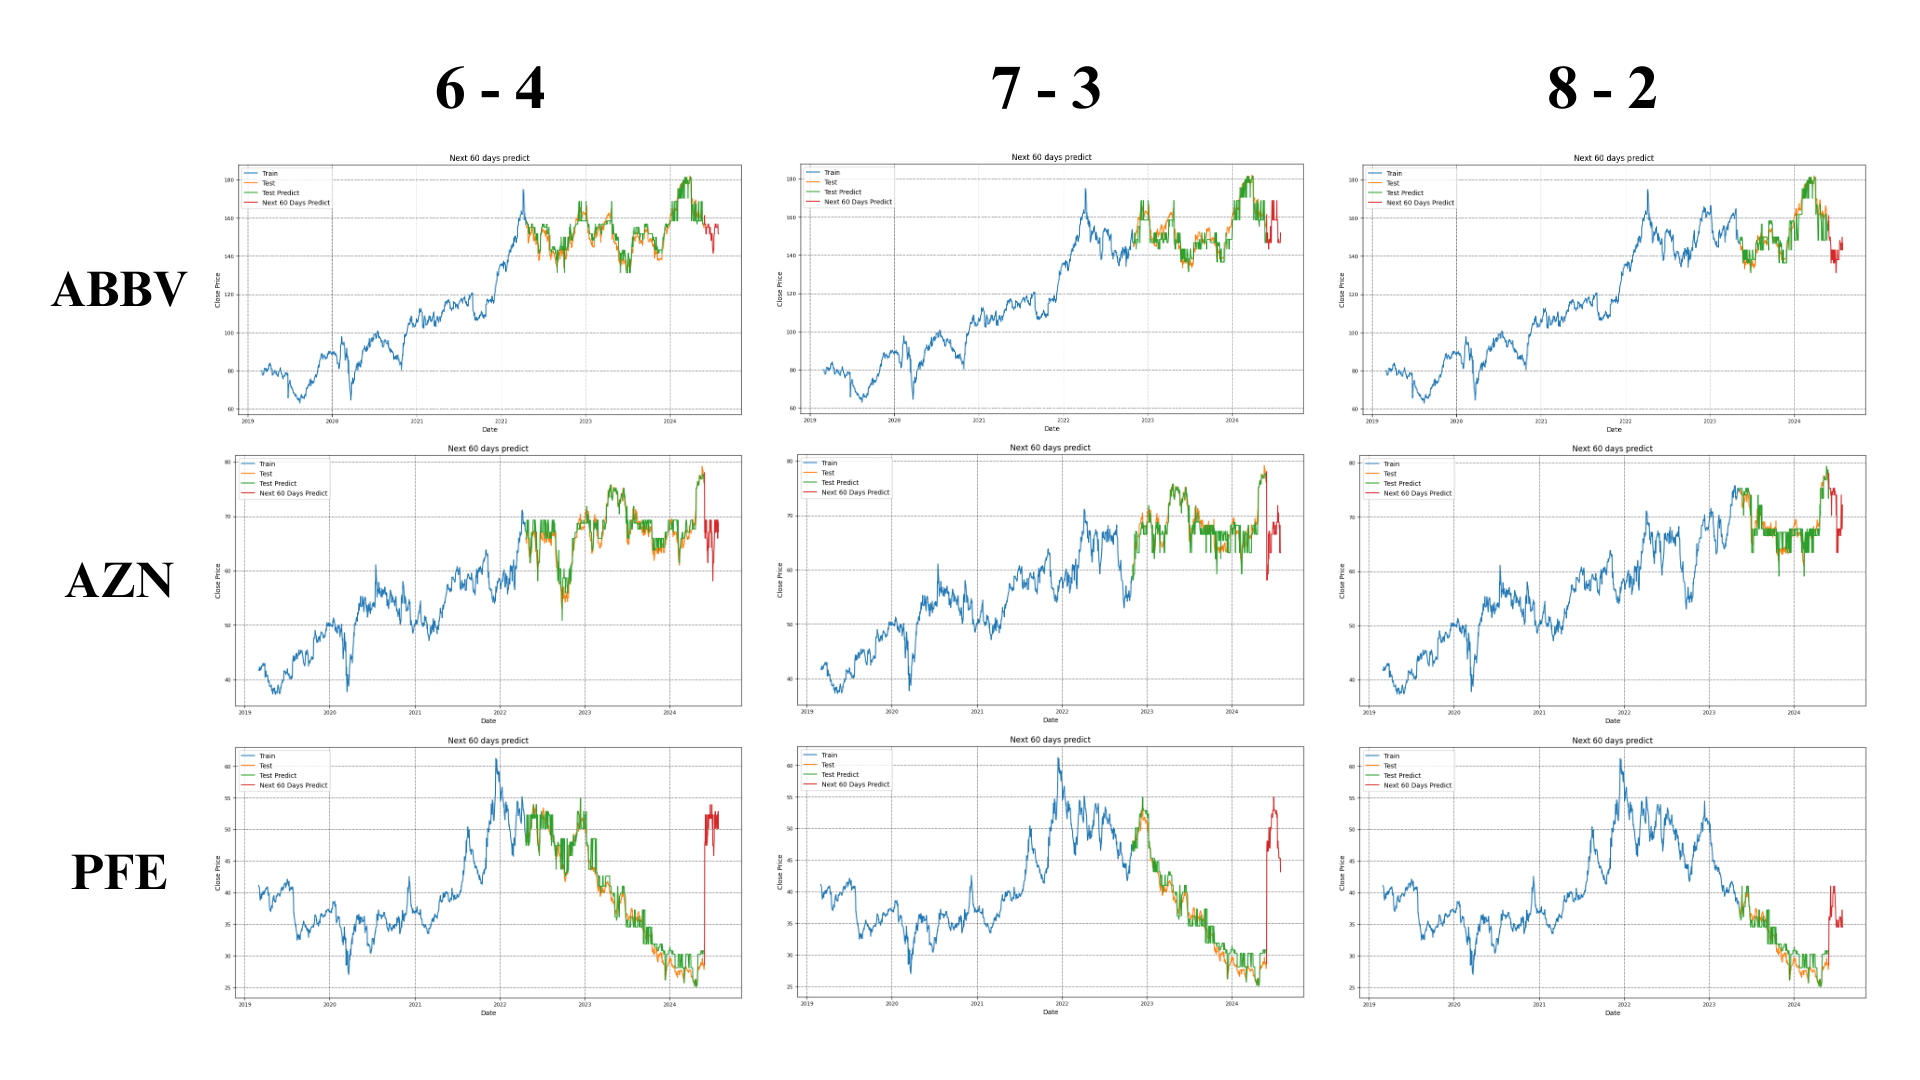
\includegraphics[width=1\textwidth]{Image/FTS60.png}
    \caption{Kết quả thực nghiệm FTS - 60 ngày}
    \label{fig:1}
    \end{minipage}
\end{figure}
\begin{figure}[H]
    \centering
    \begin{minipage}{0.5\textwidth}
    \centering
    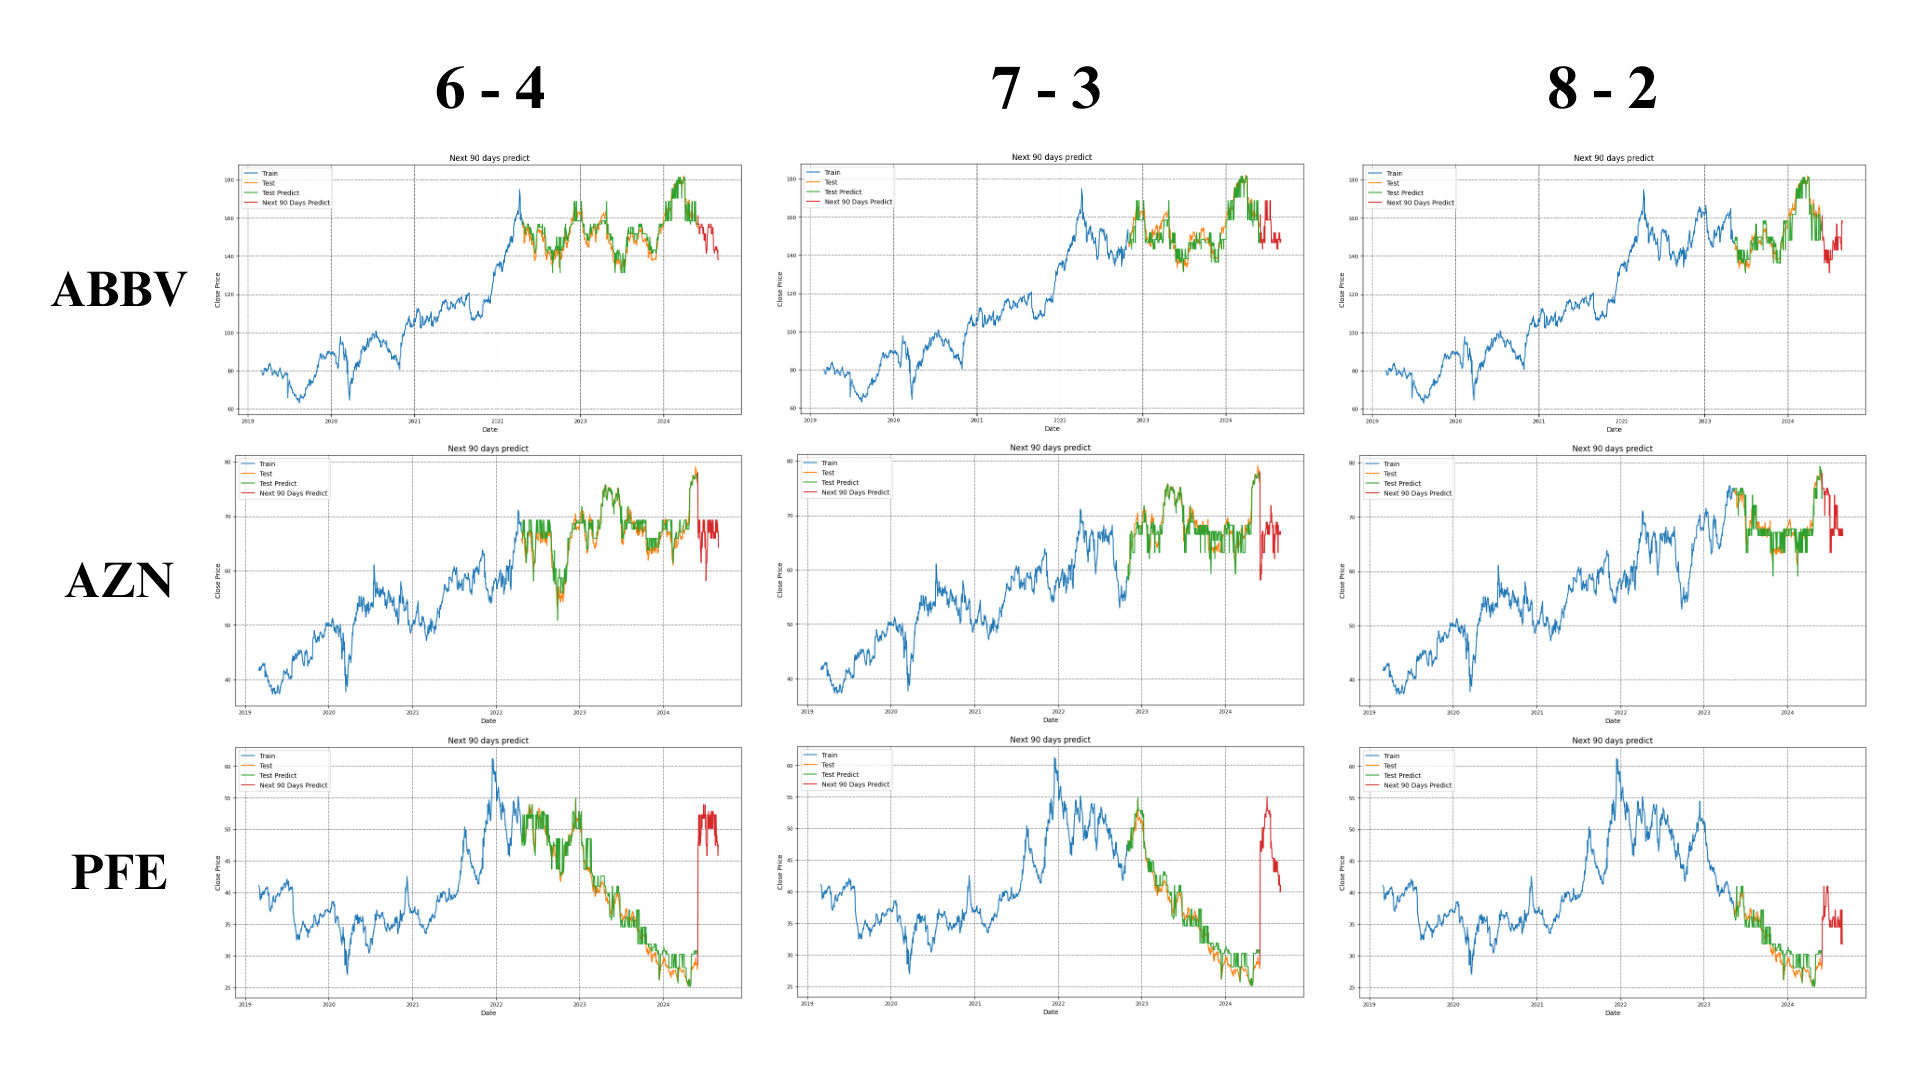
\includegraphics[width=1\textwidth]{Image/FTS90.png}
    \caption{Kết quả thực nghiệm FTS - 90 ngày}
    \label{fig:1}
    \end{minipage}
\end{figure}
\subsubsection{SEMOS}
\begin{figure}[H]
    \centering
    \begin{minipage}{0.5\textwidth}
    \centering
    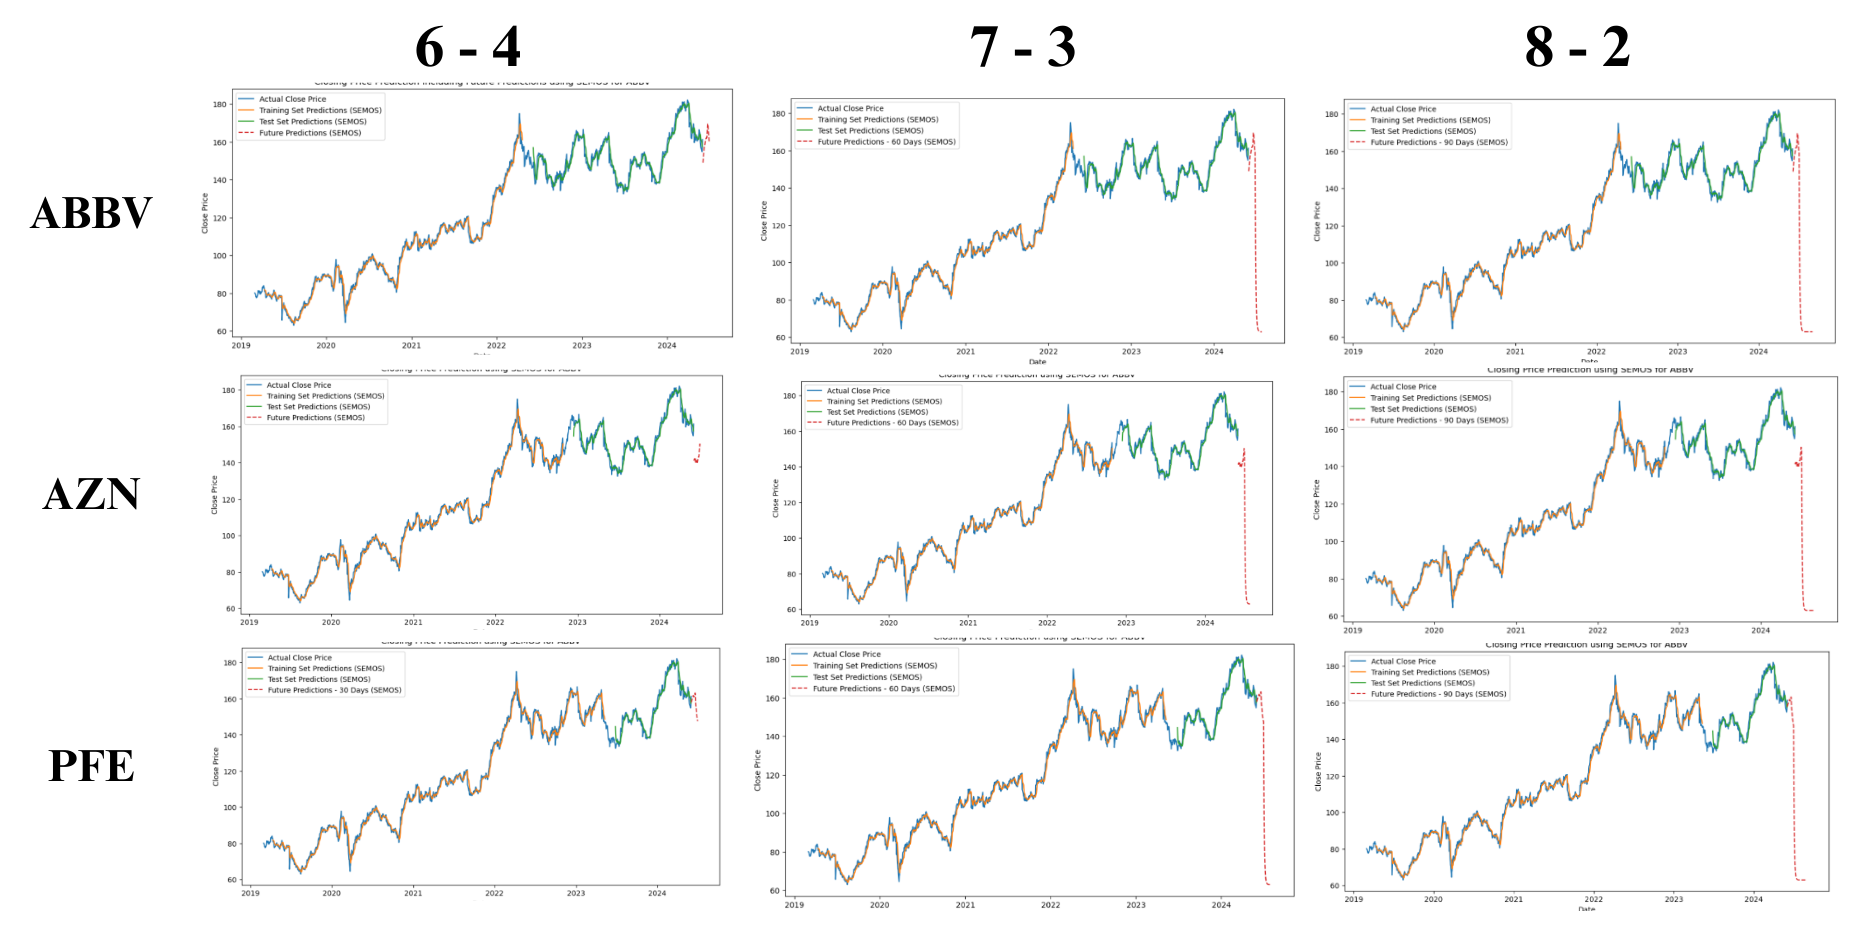
\includegraphics[width=1\textwidth]{Image/SEMOS30.png}
    \caption{Kết quả thực nghiệm SEMOS - 30 ngày}
    \label{fig:1}
    \end{minipage}
\end{figure}
\subsubsection{LIGHTGBMMODEL}
\begin{figure}[H]
    \centering
    \begin{minipage}{0.5\textwidth}
    \centering
    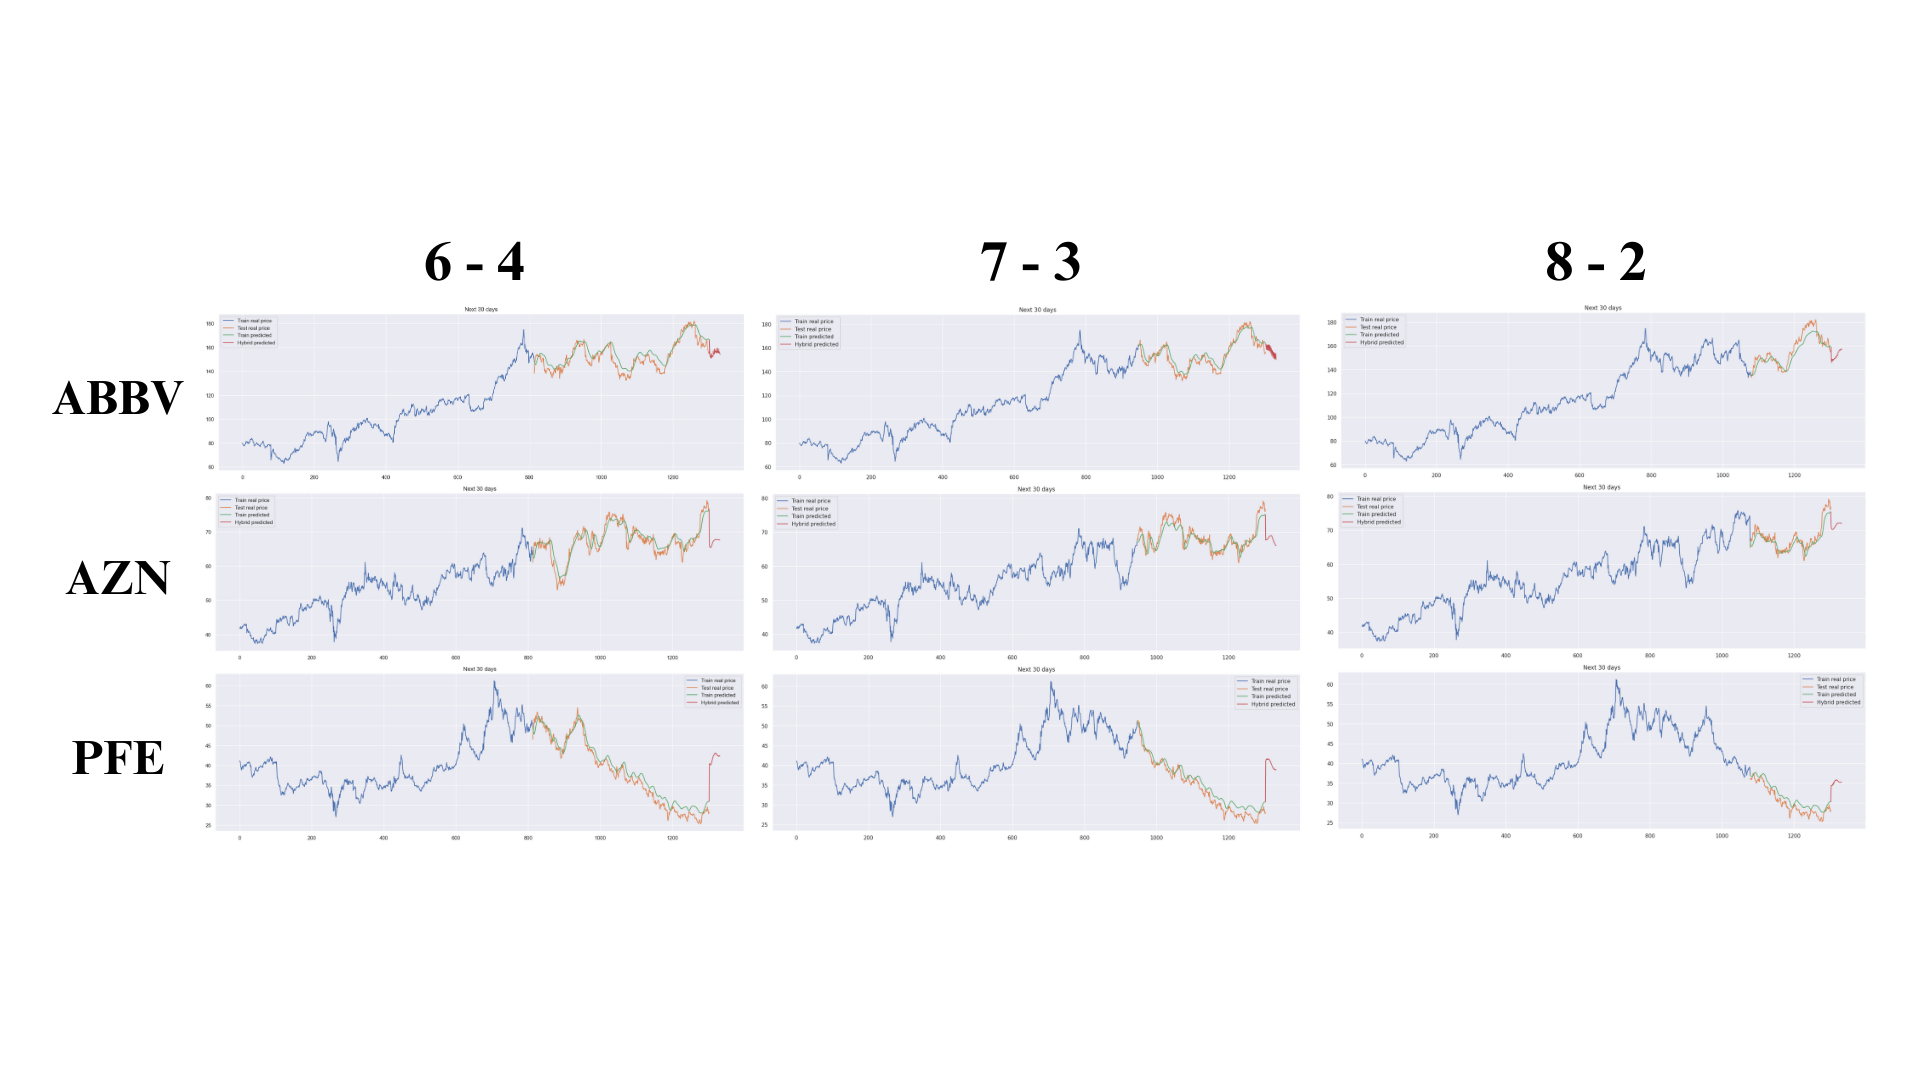
\includegraphics[width=1\textwidth]{Image/LIGHT30.png}
    \caption{Kết quả thực nghiệm LIGHTGBMMODEL - 30 ngày}
    \label{fig:1}
    \end{minipage}
\end{figure}
\begin{figure}[H]
    \centering
    \begin{minipage}{0.5\textwidth}
    \centering
    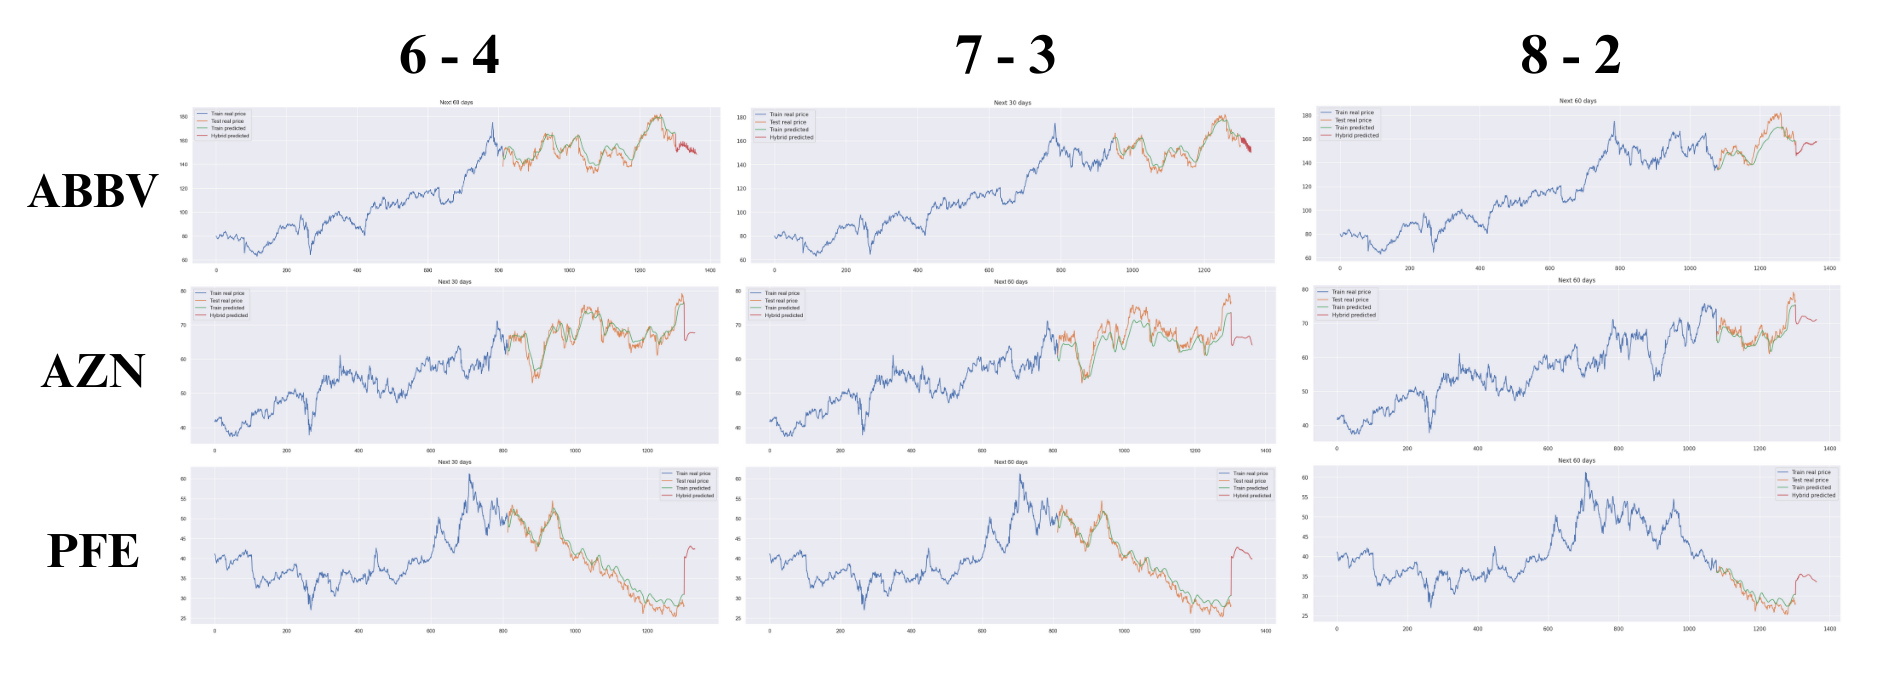
\includegraphics[width=1\textwidth]{Image/LIGHT60.png}
    \caption{Kết quả thực nghiệm LIGHTGBMMODEL - 60 ngày}
    \label{fig:1}
    \end{minipage}
\end{figure}
\begin{figure}[H]
    \centering
    \begin{minipage}{0.5\textwidth}
    \centering
    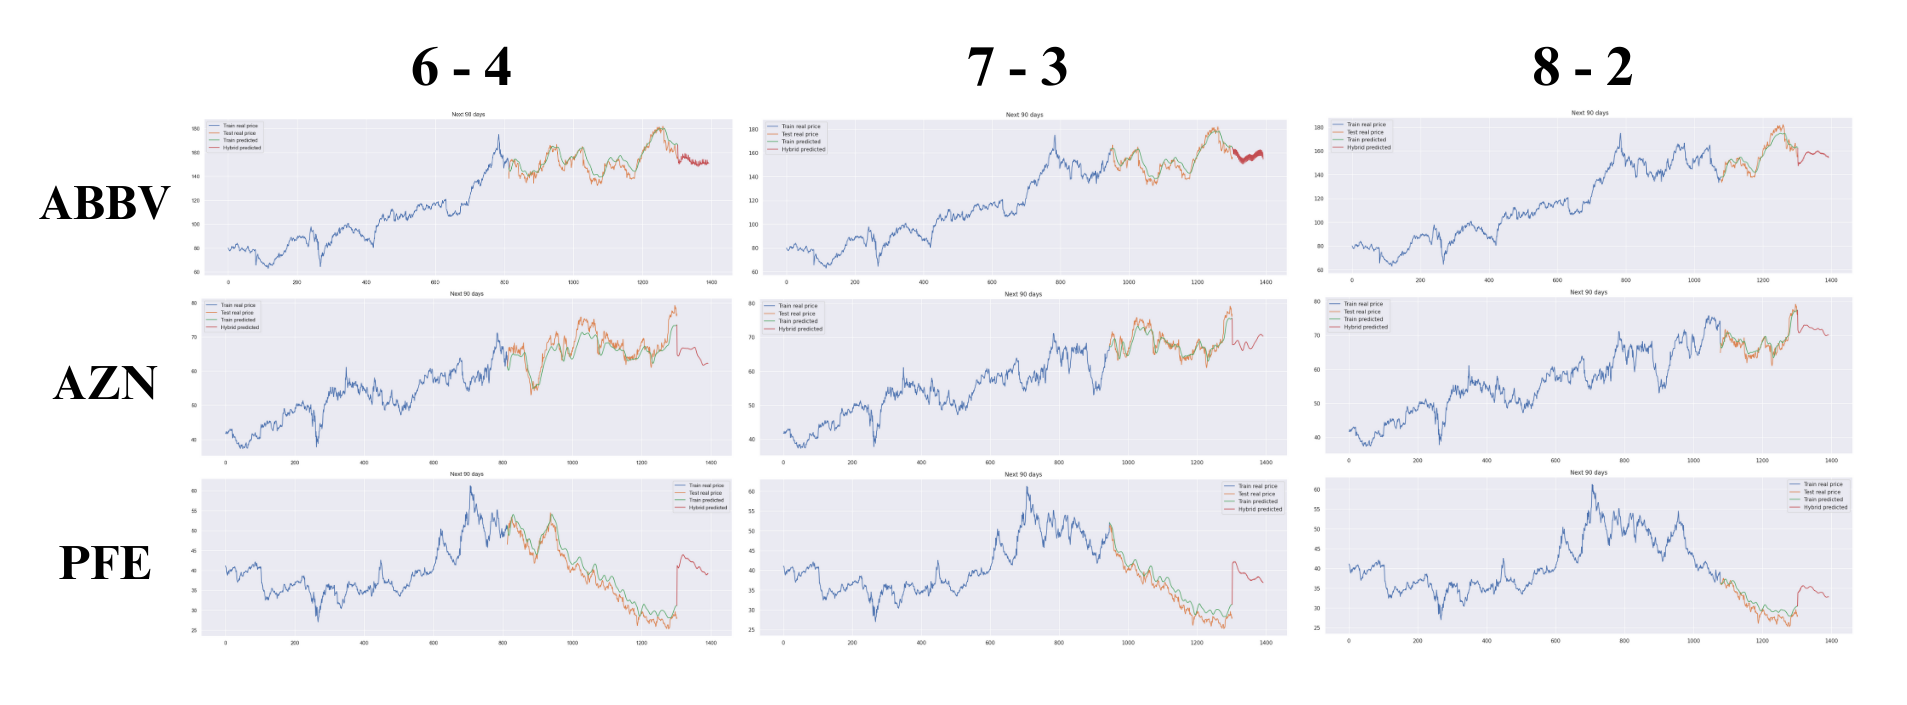
\includegraphics[width=1\textwidth]{Image/LIGHT90.png}
    \caption{Kết quả thực nghiệm LIGHTGBMMODEL - 90 ngày}
    \label{fig:1}
    \end{minipage}
\end{figure}
\subsubsection{RESCNN}
\begin{figure}[H]
    \centering
    \begin{minipage}{0.5\textwidth}
    \centering
    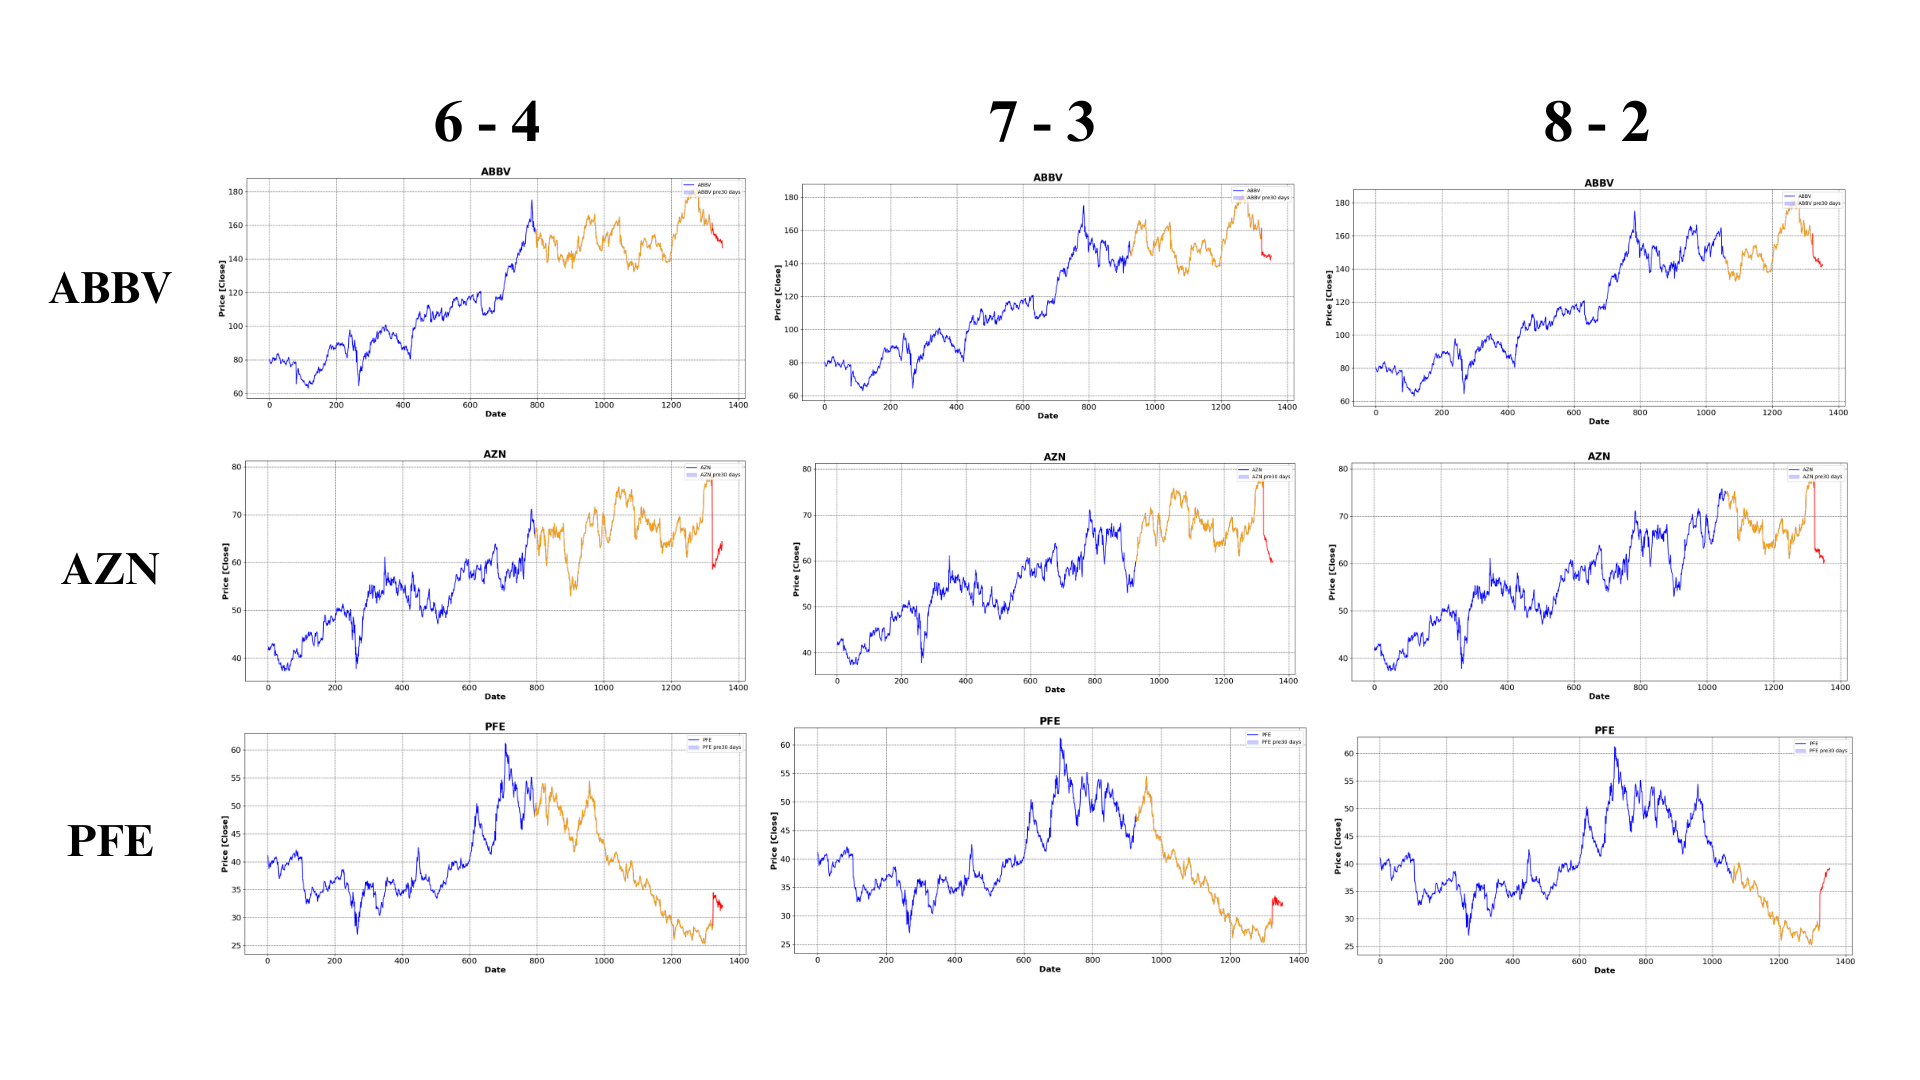
\includegraphics[width=1\textwidth]{Image/RESCNN30.png}
    \caption{Kết quả thực nghiệm RESCNN - 30 ngày}
    \label{fig:1}
    \end{minipage}
\end{figure}
\begin{figure}[H]
    \centering
    \begin{minipage}{0.5\textwidth}
    \centering
    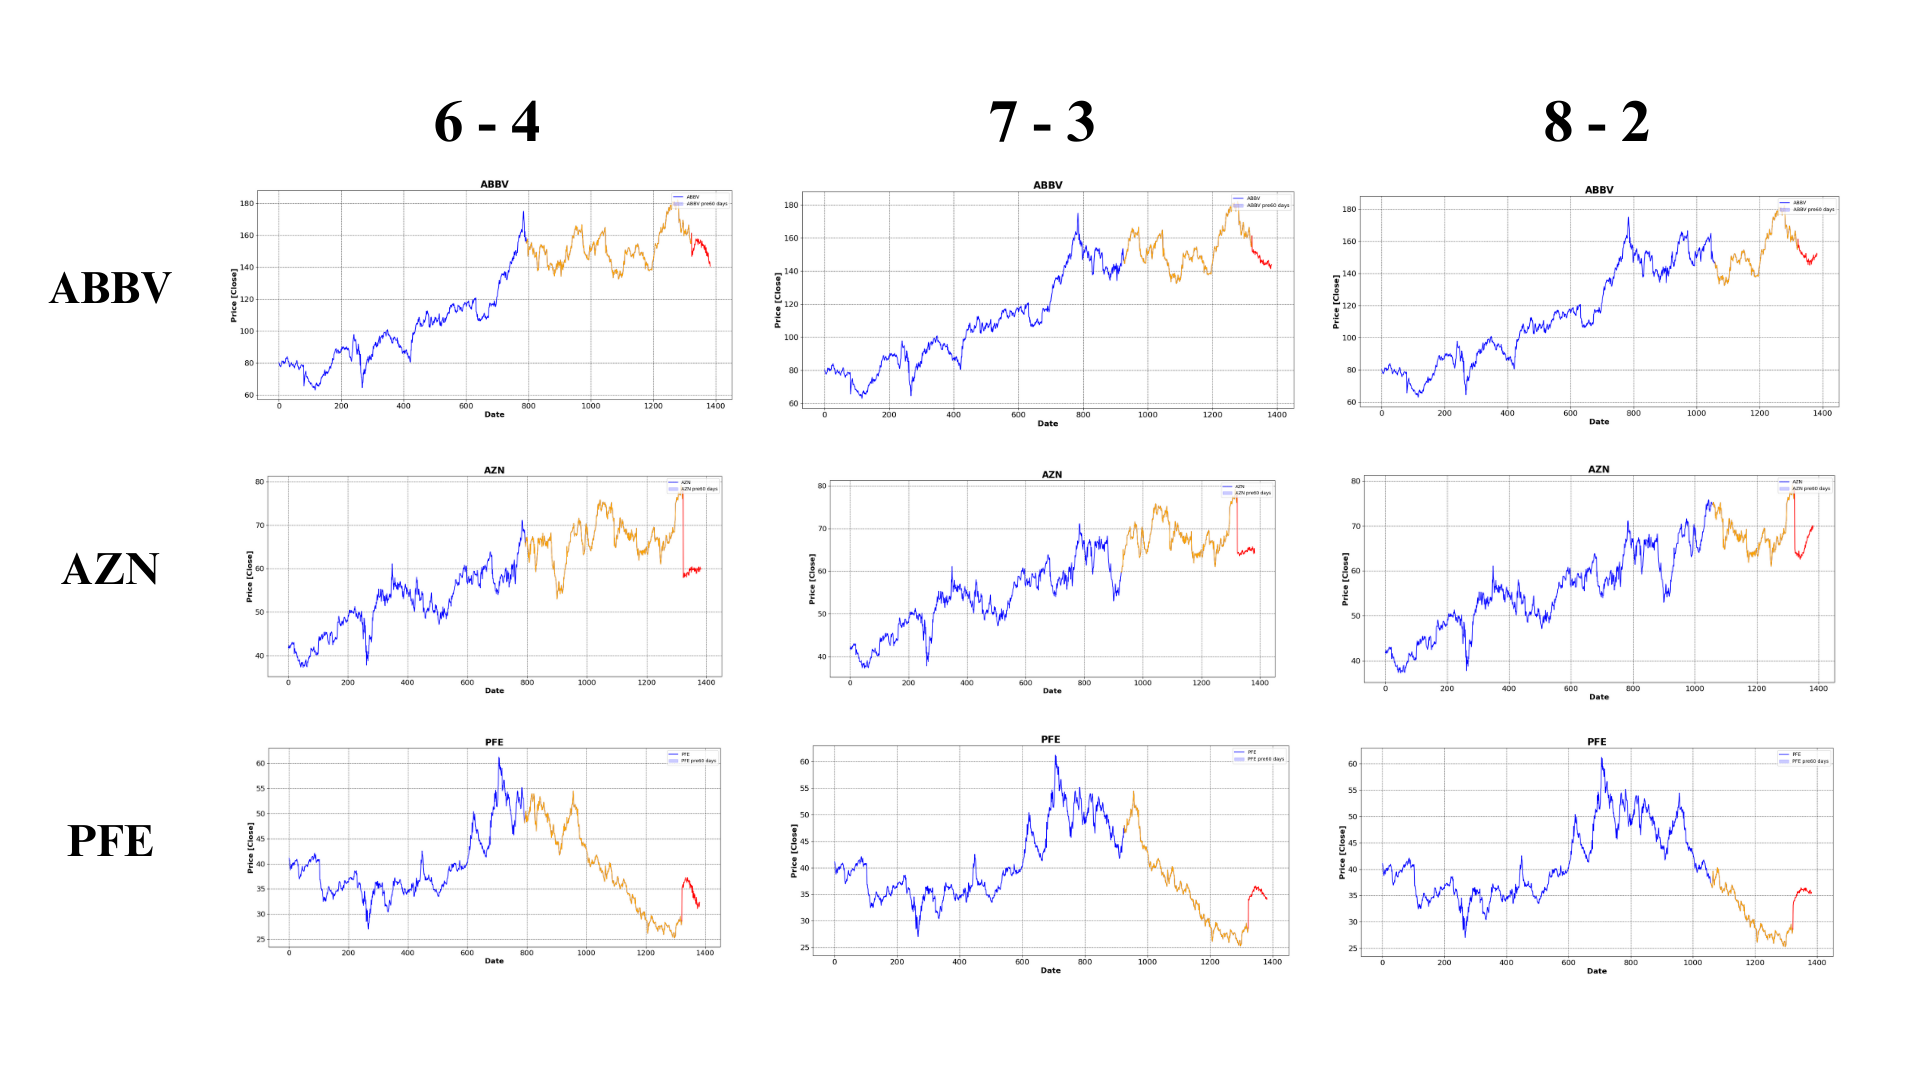
\includegraphics[width=1\textwidth]{Image/RESCNN60.png}
    \caption{Kết quả thực nghiệm RESCNN - 60 ngày}
    \label{fig:1}
    \end{minipage}
\end{figure}
\begin{figure}[H]
    \centering
    \begin{minipage}{0.5\textwidth}
    \centering
    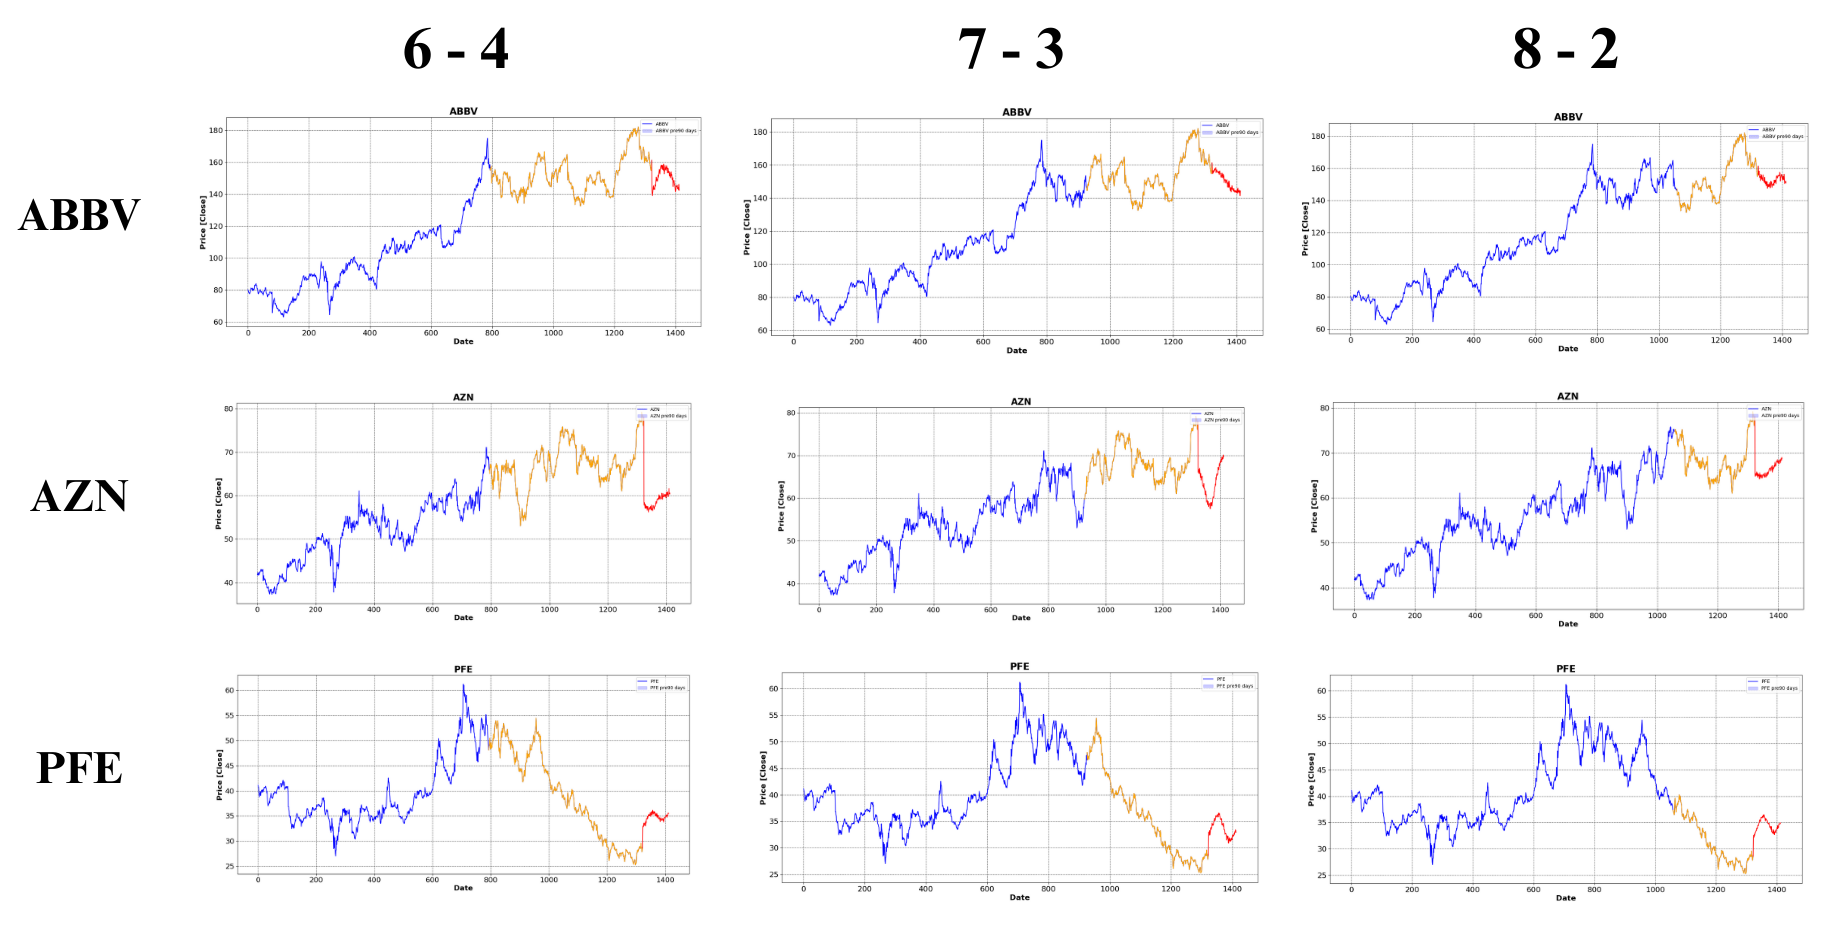
\includegraphics[width=1\textwidth]{Image/RESCNN90.png}
    \caption{Kết quả thực nghiệm RESCNN - 90 ngày}
    \label{fig:1}
    \end{minipage}
\end{figure}
Kết quả thực nghiệm sau khi thu thập được đánh giá dựa trên ba độ đo và đề cập dưới bảng sau:
\begin{table}[H]
    \centering
    \caption{Đánh giá kết quả thực nghiệm}
    \renewcommand{\arraystretch}{2}
    \tiny
    \begin{adjustbox}{width=0.5\textwidth}
    \begin{tabular}{|c|c|c|c|c|c|c|c|c|c|c|} \hline
          \multicolumn{2}{|c|}{Dataset} & \multicolumn{3}{c|}{ABBV} & \multicolumn{3}{c|}{AZN} & \multicolumn{3}{c|}{PFE} \\ \cline{1-11}
          \multicolumn{2}{|c|}{Tỷ lệ chia} & 8:2 & 7:3 & 6:4 & 8:2 & 7:3 & 6:4 & 8:2 & 7:3 & 6:4 \\ \hline
         Mô hình & Độ đo & & & & & & & & & \\ \hline
         \multirow{3}{*}{LR} & RMSE & 21,388 & 18,116 & 14,73 & 6,185 & 5,04 & 5,612 & 20,195 & 19,74 & 16,978 \\ \cline{2-11}
         & MAE & 19,277 & 15,012 & 11,84 & 5,359 & 4,29 & 4,59 & 19,504 & 17,43 & 13,716 \\ \cline{2-11}
         & MAPE & 0,13 & 0,1 & 0,0796 & 0,08 & 0,06 & 0,0707 & 0,653 & 0,56 & 0,433 \\ \cline{2-11} \hline
         \multirow{3}{*}{GRU} & RMSE & 151,229 & 150,204 & 149,918 & 65,534 & 67,294 & 65,811 & 31,44 & 35,309 & 39,235 \\ \cline{2-11}
         & MAE & 150,893 & 149,86 & 149,59 & 65,496 & 67,205 & 65,657 & 31,285 & 34,953 & 38,583 \\ \cline{2-11}
         & MAPE & 19675,9 & 20115,857 & 20188,16 & 8691,35 & 8515,425 & 8892,012 & inf & inf & inf \\ \cline{2-11} \hline
         \multirow{3}{*}{ARIMA} & RMSE & 15,785 & 14,413 & 35,4 & 7,419 & 10,44 & 4,84 & 7,466 & 13,15 & 13,126 \\ \cline{2-11}
         & MAE & 12,28 & 11,25 & 32,4 & 6,638 & 9,649 & 3,549 & 6,39 & 11,569 & 10,68 \\ \cline{2-11}
         & MAPE & 0,076 & 0,07 & 0,216 & 0,1 & 0,138 & 0,054 & 0,223 & 0,373 & 0,336 \\ \cline{2-11} \hline
         \multirow{3}{*}{LTSM} & \textbf{RMSE} & \textbf{0,034} & \textbf{0,036} & \textbf{0,032} & \textbf{0,027} & \textbf{0,028} & \textbf{0,038} & \textbf{0,019} & \textbf{0,023} & \textbf{0,036} \\ \cline{2-11}
         & \textbf{MAE} & \textbf{0,027} & \textbf{0,03} & \textbf{0,024} & \textbf{0,0197} & \textbf{0,0203} & \textbf{0,029} & \textbf{0,015} & \textbf{0,018} & \textbf{0,028} \\ \cline{2-11}
         & MAPE & 0,036 & 0,038 & 0,033 & 0,027 & 0,028 & 0,043 & 47,25.$10^9$ & 7,41.$10^9$ & 28,75.$10^9$ \\ \cline{2-11} \hline
         \multirow{3}{*}{RNN} & RMSE & 5,952 & 4,352 & 4,71 & 1,39 & 1,51 & 1,9 & 0,888 & 1,172 & 1,146 \\ \cline{2-11}
         & MAE & 4,961 & 3,622 & 3,623 & 1,024 & 1,19 & 1,57 & 0,705 & 0,89 & 0,873 \\ \cline{2-11}
         & MAPE & 0,031 & 0,023 & 0,024 & 0,015 & 0,017 & 0,023 & 0,022 & 0,024 & 0,022 \\ \cline{2-11} \hline
         \multirow{3}{*}{RF} & RMSE & 7,5  & 12 & 11,4 & 1,5 & 4,8 & 3,3 & 2,1 & 1,3 & 1,9 \\ \cline{2-11}
         & MAE & 5 & 7,8 & 9,4 & 1,2 & 3,3 & 2,4 & 1,8 & 1 & 1,4 \\ \cline{2-11}
         & MAPE & 0,02 & 0,04 & 0,06 & 0,01 & 0,04 & 0,03 & 0,06 & 0,03 & 0,04 \\ \cline{2-11} \hline
         \multirow{3}{*}{FTS} & RMSE & 5,875  & 5,038 & 4,088 & 2,026 & 1,968 & 1,721 & 1,604 & 1,541 & 1,840 \\ \cline{2-11}
         & MAE & 34,52 & 25,38 & 16,71 & 4,106 & 3,874 & 2,965 & 2,572 & 2,375 & 3,386 \\ \cline{2-11}
         & MAPE & 0,029 & 0,027 & 0,022 & 0,023 & 0,024 & 0,021 & 0,045 & 0,039 & 0,040 \\ \cline{2-11} \hline
         \multirow{3}{*}{LightGBM} & RMSE & 5,56  & 4,42 & 5,15 & 1,66 & 1,66 & 1,73 & 2,07 & 1,61 & 1,63 \\ \cline{2-11}
         & MAE & 4,31 & 3,38 & 4,07 & 1,28 & 1,24 & 1,32 & 1,61 & 1,23 & 1,23 \\ \cline{2-11}
         & \textbf{MAPE} & \textbf{0,004} & \textbf{0,004} & \textbf{0,005} & \textbf{0,001} & \textbf{0,001} & \textbf{0,002} & \textbf{0,002} & \textbf{0,001} & \textbf{0,002} \\ \cline{2-11} \hline
         \multirow{3}{*}{ResCNN} & RMSE & 13,6  & 13,282 & 9,785 & 6,419 & 6,35 & 10,048 & 4,038 & 3,645 & 4,272 \\ \cline{2-11}
         & MAE & 11,78 & 11,633 & 8,38 & 5,59 & 5,218 & 9,134 & 3,336 & 2,946 & 3,499 \\ \cline{2-11}
         & MAPE & 0,084 & 0,078 & 0,054 & 0,0896 & 0,082 & 0,159 & 0,096 & 0,074 & 0,0869 \\ \cline{2-11} \hline
    \end{tabular}
    \end{adjustbox}
\end{table}
Bảng trên ghi nhận các giá trị độ đo RMSE, MAE, MAPE của các mô hình Random Forest (RF), Fuzzy for predict times series (FTS), 
LightGBMModel, ResCNN, Linear regression, Autoregressive Integrated Moving Average (ARIMA), Recurrent Neural Networks (RNN), Gated recurrent units (GRU)
và Long Short-Term Memory (LSTM) trên tập test của ba bộ dữ liệu ABBV, AZN và PFE
theo BA tỉ lệ của train:test là 6:4 , 7:3 và 8:2

Long Short-Term Memory (LSTM) là mô hình cho giá trị Root Mean Square Error (RMSE) và Mean Absolute Error (MAE) thấp nhất trên cả ba bộ dữ liệu 
và cũng như với ba tỉ lệ train:test.

LightGBMModel (LightGBM) đạt được giá trị Mean Absolute Percentage Error (MAPE) thấp nhất trên cả ba bộ dữ liệu và 
cũng như với ba tỉ lệ train:test.

Tổng kết lại, từ các phân tích về các độ đo lỗi như MAPE, RMSE và MSE trên cả ba bộ dữ liệu và hai tỉ lệ train:test, 
nhóm nhận thấy hai mô hình phù hợp nhất là Long Short-Term Memory (LSTM) và LightGBMModel (LightGBM). 
Cả hai mô hình này đã cho kết quả tốt nhất trong các độ đo lỗi khác nhau trên hầu hết ba bộ dữ liệu và các tỉ lệ train:test.

\section{KẾT LUẬN}
Trong bài báo này, chúng tôi đã tiến hành nghiên cứu về việc sử dụng kỹ thuật phân tích chuỗi thời gian để dự đoán giá cổ phiếu. 
Chúng tôi đã sử dụng các mô hình như SEMOS, Random Forest, Fuzzy for predict times series, LightGBMModel, ResCNN, Linear regression, 
ARIMA, RNN, GRU, LTSM trên ba bộ dữ liệu khác nhau để đưa ra dự đoán giá cổ phiếu. 
Điều này giúp chúng tôi đánh giá hiệu suất và so sánh các mô hình dự đoán. Kết quả thực nghiệm cho thấy mô hình 
và đã cho thấy hiệu suất tốt hơn so với các mô hình khác trong việc dự đoán giá cổ phiếu. 
Điều này đều chỉ ra tiềm năng của các mô hình kỹ thuật phân tích chuỗi thời gian trong lĩnh vực dự đoán giá cổ phiếu.

Mặc dù đã đạt được một số kết quả khả quan, quá trình nghiên cứu không tránh khỏi một số khó khăn. 
Một trong những khó khăn là tính phức tạp và biến động của thị trường tài chính, làm tăng độ khó trong việc dự đoán giá cổ phiếu. 

Trong tương lai, chúng tôi sẽ tiếp tục nghiên cứu, áp dụng các kỹ thuật trong tinh chỉnh mô hình để cải tiến các mô hình 
dự đoán giá cổ phiếu. Ngoài ra chúng tôi có thể nghiên cứu và áp dụng các mô hình mới nhất và phát triển phương pháp kết hợp 
giữa các mô hình khác nhau để tăng độ chính xác và tin cậy của dự đoán. Đồng thời, mở rộng phạm vi nghiên cứu bằng cách sử dụng 
thêm nhiều dữ liệu từ các thị trường tài chính khác nhau như tin tức, sự kiện và thông tin khác để dự đoán chính xác hơn.

\begin{thebibliography}{00}
\bibitem{b1} Zou Xiaowu, Wang Zidong, Li Qi, Sheng Weiguo ``Integration of residual network and convolutional neural network along with various activation functions and global pooling for time series classification'' ,2019. [Online]. Link: https://www.sciencedirect.com/science/article/abs/pii/S0925231219311506
\bibitem{b2} Guolin Ke, Qi Meng, Thomas Finley ``LightGBM: A Highly Efficient Gradient Boosting Decision Tree'' ,2017. [Online]. Link: https://proceedings.neurips.cc/paper\_files/paper/2017/file/...
\bibitem{b3} Mária Lakatos, Sebastian Lerch, Stephan Hemri, Sándor Baran ``Comparison of multivariate post-processing methods using global ECMWF ensemble forecasts'' ,2023. [Online]. Link: https://rmets.onlinelibrary.wiley.com/doi/full/10.1002/qj.4436
\bibitem{b4}
\bibitem{b5} Gang Liu, Fuyuan Xiao, ... (2020) ``A Fuzzy Interval Time-Series Energy and Financial Forecasting Model Using Network-Based Multiple Time-Frequency Spaces and the Induced-Ordered Weighted Averaging Aggregation Operation''.[Online]. Link: https://ieeexplore.ieee.org/abstract/document/8988162
\bibitem{b6} Gururaj, V., Shriya, V. R., \& Ashwini, K. (2019). Stock market prediction using linear regression and support vector machines. Int J Appl Eng Res, 14(8), 1931-1934.
\bibitem{b7} Disha, R. A., \& Waheed, S. (2022). Performance analysis of machine learning models for intrusion detection system using Gini Impurity-based Weighted Random Forest (GIWRF) feature selection technique. Cybersecurity, 5(1), 1-20
\bibitem{b8} A. A. Ariyo, A. O. Adewumi and C. K. Ayo, "Stock Price Prediction Using the ARIMA Model," 2014 UKSim-AMSS 16th International Conference on Computer Modelling and Simulation, Cambridge, UK, 2014, pp. 106-112, doi: 10.1109/UKSim.2014.67.
\bibitem{b9} A. Meyler, G. Kenny and T. Quinn, “Forecasting Irish Inflation using ARIMA Models”, Central Bank of Ireland Research Department, Technical Paper, 3/RT/1998.
\bibitem{b10} Roondiwala, M., Patel, H., \& Varma, S. (2017, April). Predicting Stock Prices Using LSTM. IJSC publishing.
\bibitem{b11}	Yongqiong Zhu. 2020. Stock price prediction using the RNN model. 2020 International Conference on Applied Physics and Computing (ICAPC 2020). IOP Publishing.
\end{thebibliography}
\end{document}
